\documentclass[a4paper]{article}
\usepackage[margin=0.5in]{geometry}
\usepackage{booktabs}
\usepackage{tikz}
\usepackage{ytableau}
\usepackage{hyperref}
\usepackage{fancyhdr}
\usepackage{multicol}
\usepackage{titlesec}
\pagestyle{fancy}
\fancyhf{}
\fancyhead[L]{NumericalSemigroup Catalog}
\fancyfoot[C]{\thepage}
\titleformat{\section}{\normalfont\Large\bfseries}{}{0em}{}
\titleformat{\subsection}{\normalfont\large\bfseries}{}{0em}{}
\titlespacing*{\section}{0pt}{12pt plus 4pt minus 2pt}{0pt plus 2pt minus 2pt}
\titlespacing*{\subsection}{0pt}{12pt plus 4pt minus 2pt}{0pt plus 2pt minus 2pt}
\begin{document}
\tableofcontents
\newpage
\newpage\subsection{[2, 7]}
\noindent\begin{minipage}{0.6\textwidth}
\subsubsection*{Invariants}
\centering
\begin{tabular}{|c|c|c|c|c|c|c|}
\toprule
g & F & m & ewt & t & \(|M|\) & \(|\lambda|\) \\
\midrule
3 & 5 & 2 & 2 & 1 & 0 & 6 \\
\bottomrule
\end{tabular}
\end{minipage}%
\begin{minipage}{0.4\textwidth}
\subsubsection*{Partition}
\centering
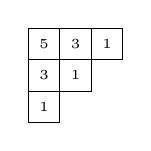
\begin{tikzpicture}
  \draw (0.00, 0.00) rectangle (0.40, -0.40);
  \node[font=\tiny] at (0.20, -0.20) {5};
  \draw (0.40, 0.00) rectangle (0.80, -0.40);
  \node[font=\tiny] at (0.60, -0.20) {3};
  \draw (0.80, 0.00) rectangle (1.20, -0.40);
  \node[font=\tiny] at (1.00, -0.20) {1};
  \draw (0.00, -0.40) rectangle (0.40, -0.80);
  \node[font=\tiny] at (0.20, -0.60) {3};
  \draw (0.40, -0.40) rectangle (0.80, -0.80);
  \node[font=\tiny] at (0.60, -0.60) {1};
  \draw (0.00, -0.80) rectangle (0.40, -1.20);
  \node[font=\tiny] at (0.20, -1.00) {1};
\end{tikzpicture}
\end{minipage}
\vspace{1cm}
\noindent \newline\begin{minipage}{0.48\textwidth}
\subsubsection*{Gap Poset}
\centering
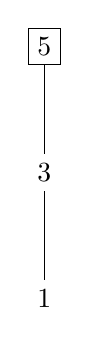
\begin{tikzpicture}
  \node[minimum size=0.3cm] (1) at (0.00,-3.20) {1};
  \node[minimum size=0.3cm] (3) at (0.00,-1.60) {3};
  \node[draw, rectangle, minimum size=0.3cm] (5) at (0.00,0.00) {5};
  % Draw the cover relations
  \draw (3) -- (1);
  \draw (5) -- (3);
\end{tikzpicture}
\end{minipage}%
\hfill\begin{minipage}{0.48\textwidth}
\subsubsection*{Void Poset}
\centering
\end{minipage}
\newpage\subsection{[3, 5]}
\noindent\begin{minipage}{0.6\textwidth}
\subsubsection*{Invariants}
\centering
\begin{tabular}{|c|c|c|c|c|c|c|}
\toprule
g & F & m & ewt & t & \(|M|\) & \(|\lambda|\) \\
\midrule
4 & 7 & 3 & 3 & 1 & 0 & 8 \\
\bottomrule
\end{tabular}
\end{minipage}%
\begin{minipage}{0.4\textwidth}
\subsubsection*{Partition}
\centering
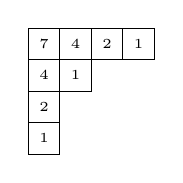
\begin{tikzpicture}
  \draw (0.00, 0.00) rectangle (0.40, -0.40);
  \node[font=\tiny] at (0.20, -0.20) {7};
  \draw (0.40, 0.00) rectangle (0.80, -0.40);
  \node[font=\tiny] at (0.60, -0.20) {4};
  \draw (0.80, 0.00) rectangle (1.20, -0.40);
  \node[font=\tiny] at (1.00, -0.20) {2};
  \draw (1.20, 0.00) rectangle (1.60, -0.40);
  \node[font=\tiny] at (1.40, -0.20) {1};
  \draw (0.00, -0.40) rectangle (0.40, -0.80);
  \node[font=\tiny] at (0.20, -0.60) {4};
  \draw (0.40, -0.40) rectangle (0.80, -0.80);
  \node[font=\tiny] at (0.60, -0.60) {1};
  \draw (0.00, -0.80) rectangle (0.40, -1.20);
  \node[font=\tiny] at (0.20, -1.00) {2};
  \draw (0.00, -1.20) rectangle (0.40, -1.60);
  \node[font=\tiny] at (0.20, -1.40) {1};
\end{tikzpicture}
\end{minipage}
\vspace{1cm}
\noindent \newline\begin{minipage}{0.48\textwidth}
\subsubsection*{Gap Poset}
\centering
\begin{tikzpicture}
  \node[minimum size=0.3cm] (1) at (0.00,-3.20) {1};
  \node[minimum size=0.3cm] (2) at (0.00,-1.60) {2};
  \node[minimum size=0.3cm] (4) at (1.60,-1.60) {4};
  \node[draw, rectangle, minimum size=0.3cm] (7) at (0.00,0.00) {7};
  % Draw the cover relations
  \draw (7) -- (4);
  \draw (4) -- (1);
  \draw (7) -- (2);
\end{tikzpicture}
\end{minipage}%
\hfill\begin{minipage}{0.48\textwidth}
\subsubsection*{Void Poset}
\centering
\end{minipage}
\newpage\subsection{[4, 6, 7]}
\noindent\begin{minipage}{0.6\textwidth}
\subsubsection*{Invariants}
\centering
\begin{tabular}{|c|c|c|c|c|c|c|}
\toprule
g & F & m & ewt & t & \(|M|\) & \(|\lambda|\) \\
\midrule
5 & 9 & 4 & 4 & 1 & 0 & 10 \\
\bottomrule
\end{tabular}
\end{minipage}%
\begin{minipage}{0.4\textwidth}
\subsubsection*{Partition}
\centering
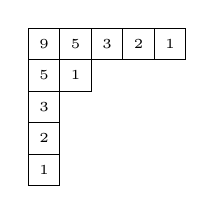
\begin{tikzpicture}
  \draw (0.00, 0.00) rectangle (0.40, -0.40);
  \node[font=\tiny] at (0.20, -0.20) {9};
  \draw (0.40, 0.00) rectangle (0.80, -0.40);
  \node[font=\tiny] at (0.60, -0.20) {5};
  \draw (0.80, 0.00) rectangle (1.20, -0.40);
  \node[font=\tiny] at (1.00, -0.20) {3};
  \draw (1.20, 0.00) rectangle (1.60, -0.40);
  \node[font=\tiny] at (1.40, -0.20) {2};
  \draw (1.60, 0.00) rectangle (2.00, -0.40);
  \node[font=\tiny] at (1.80, -0.20) {1};
  \draw (0.00, -0.40) rectangle (0.40, -0.80);
  \node[font=\tiny] at (0.20, -0.60) {5};
  \draw (0.40, -0.40) rectangle (0.80, -0.80);
  \node[font=\tiny] at (0.60, -0.60) {1};
  \draw (0.00, -0.80) rectangle (0.40, -1.20);
  \node[font=\tiny] at (0.20, -1.00) {3};
  \draw (0.00, -1.20) rectangle (0.40, -1.60);
  \node[font=\tiny] at (0.20, -1.40) {2};
  \draw (0.00, -1.60) rectangle (0.40, -2.00);
  \node[font=\tiny] at (0.20, -1.80) {1};
\end{tikzpicture}
\end{minipage}
\vspace{1cm}
\noindent \newline\begin{minipage}{0.48\textwidth}
\subsubsection*{Gap Poset}
\centering
\begin{tikzpicture}
  \node[minimum size=0.3cm] (1) at (0.00,-3.20) {1};
  \node[minimum size=0.3cm] (2) at (0.00,-1.60) {2};
  \node[minimum size=0.3cm] (3) at (1.60,-1.60) {3};
  \node[minimum size=0.3cm] (5) at (3.20,-1.60) {5};
  \node[draw, rectangle, minimum size=0.3cm] (9) at (0.00,0.00) {9};
  % Draw the cover relations
  \draw (9) -- (5);
  \draw (9) -- (2);
  \draw (5) -- (1);
  \draw (9) -- (3);
\end{tikzpicture}
\end{minipage}%
\hfill\begin{minipage}{0.48\textwidth}
\subsubsection*{Void Poset}
\centering
\end{minipage}
\newpage\subsection{[3, 7, 11]}
\noindent\begin{minipage}{0.6\textwidth}
\subsubsection*{Invariants}
\centering
\begin{tabular}{|c|c|c|c|c|c|c|}
\toprule
g & F & m & ewt & t & \(|M|\) & \(|\lambda|\) \\
\midrule
5 & 8 & 3 & 4 & 2 & 1 & 10 \\
\bottomrule
\end{tabular}
\end{minipage}%
\begin{minipage}{0.4\textwidth}
\subsubsection*{Partition}
\centering
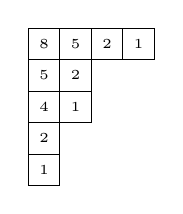
\begin{tikzpicture}
  \draw (0.00, 0.00) rectangle (0.40, -0.40);
  \node[font=\tiny] at (0.20, -0.20) {8};
  \draw (0.40, 0.00) rectangle (0.80, -0.40);
  \node[font=\tiny] at (0.60, -0.20) {5};
  \draw (0.80, 0.00) rectangle (1.20, -0.40);
  \node[font=\tiny] at (1.00, -0.20) {2};
  \draw (1.20, 0.00) rectangle (1.60, -0.40);
  \node[font=\tiny] at (1.40, -0.20) {1};
  \draw (0.00, -0.40) rectangle (0.40, -0.80);
  \node[font=\tiny] at (0.20, -0.60) {5};
  \draw (0.40, -0.40) rectangle (0.80, -0.80);
  \node[font=\tiny] at (0.60, -0.60) {2};
  \draw (0.00, -0.80) rectangle (0.40, -1.20);
  \node[font=\tiny] at (0.20, -1.00) {4};
  \draw (0.40, -0.80) rectangle (0.80, -1.20);
  \node[font=\tiny] at (0.60, -1.00) {1};
  \draw (0.00, -1.20) rectangle (0.40, -1.60);
  \node[font=\tiny] at (0.20, -1.40) {2};
  \draw (0.00, -1.60) rectangle (0.40, -2.00);
  \node[font=\tiny] at (0.20, -1.80) {1};
\end{tikzpicture}
\end{minipage}
\vspace{1cm}
\noindent \newline\begin{minipage}{0.48\textwidth}
\subsubsection*{Gap Poset}
\centering
\begin{tikzpicture}
  \node[minimum size=0.3cm] (1) at (0.00,-1.60) {1};
  \node[minimum size=0.3cm] (5) at (1.60,-1.60) {5};
  \node[minimum size=0.3cm] (2) at (1.60,-3.20) {2};
  \node[minimum size=0.3cm] (4) at (0.00,0.00) {4};
  \node[draw, rectangle, minimum size=0.3cm] (8) at (1.60,0.00) {8};
  % Draw the cover relations
  \draw (5) -- (2);
  \draw (4) -- (1);
  \draw (8) -- (5);
  \draw (8) -- (1);
\end{tikzpicture}
\end{minipage}%
\hfill\begin{minipage}{0.48\textwidth}
\subsubsection*{Void Poset}
\centering

\begin{tikzpicture}
  \node[draw, rectangle, minimum size=0.3cm] (4) at (0.00,0.00) {4};
\end{tikzpicture}
\end{minipage}
\newpage\subsection{[4, 6, 9]}
\noindent\begin{minipage}{0.6\textwidth}
\subsubsection*{Invariants}
\centering
\begin{tabular}{|c|c|c|c|c|c|c|}
\toprule
g & F & m & ewt & t & \(|M|\) & \(|\lambda|\) \\
\midrule
6 & 11 & 4 & 6 & 1 & 0 & 14 \\
\bottomrule
\end{tabular}
\end{minipage}%
\begin{minipage}{0.4\textwidth}
\subsubsection*{Partition}
\centering
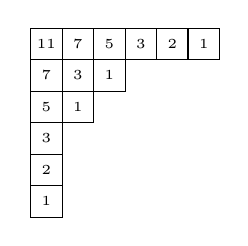
\begin{tikzpicture}
  \draw (0.00, 0.00) rectangle (0.40, -0.40);
  \node[font=\tiny] at (0.20, -0.20) {11};
  \draw (0.40, 0.00) rectangle (0.80, -0.40);
  \node[font=\tiny] at (0.60, -0.20) {7};
  \draw (0.80, 0.00) rectangle (1.20, -0.40);
  \node[font=\tiny] at (1.00, -0.20) {5};
  \draw (1.20, 0.00) rectangle (1.60, -0.40);
  \node[font=\tiny] at (1.40, -0.20) {3};
  \draw (1.60, 0.00) rectangle (2.00, -0.40);
  \node[font=\tiny] at (1.80, -0.20) {2};
  \draw (2.00, 0.00) rectangle (2.40, -0.40);
  \node[font=\tiny] at (2.20, -0.20) {1};
  \draw (0.00, -0.40) rectangle (0.40, -0.80);
  \node[font=\tiny] at (0.20, -0.60) {7};
  \draw (0.40, -0.40) rectangle (0.80, -0.80);
  \node[font=\tiny] at (0.60, -0.60) {3};
  \draw (0.80, -0.40) rectangle (1.20, -0.80);
  \node[font=\tiny] at (1.00, -0.60) {1};
  \draw (0.00, -0.80) rectangle (0.40, -1.20);
  \node[font=\tiny] at (0.20, -1.00) {5};
  \draw (0.40, -0.80) rectangle (0.80, -1.20);
  \node[font=\tiny] at (0.60, -1.00) {1};
  \draw (0.00, -1.20) rectangle (0.40, -1.60);
  \node[font=\tiny] at (0.20, -1.40) {3};
  \draw (0.00, -1.60) rectangle (0.40, -2.00);
  \node[font=\tiny] at (0.20, -1.80) {2};
  \draw (0.00, -2.00) rectangle (0.40, -2.40);
  \node[font=\tiny] at (0.20, -2.20) {1};
\end{tikzpicture}
\end{minipage}
\vspace{1cm}
\noindent \newline\begin{minipage}{0.48\textwidth}
\subsubsection*{Gap Poset}
\centering
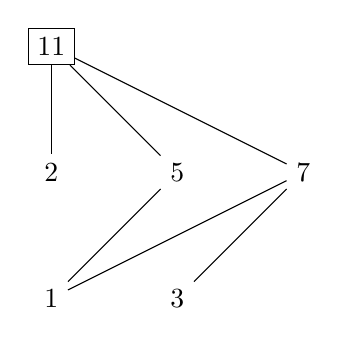
\begin{tikzpicture}
  \node[minimum size=0.3cm] (1) at (0.00,-3.20) {1};
  \node[minimum size=0.3cm] (3) at (1.60,-3.20) {3};
  \node[minimum size=0.3cm] (2) at (0.00,-1.60) {2};
  \node[minimum size=0.3cm] (5) at (1.60,-1.60) {5};
  \node[minimum size=0.3cm] (7) at (3.20,-1.60) {7};
  \node[draw, rectangle, minimum size=0.3cm] (11) at (0.00,0.00) {11};
  % Draw the cover relations
  \draw (11) -- (7);
  \draw (7) -- (1);
  \draw (5) -- (1);
  \draw (7) -- (3);
  \draw (11) -- (2);
  \draw (11) -- (5);
\end{tikzpicture}
\end{minipage}%
\hfill\begin{minipage}{0.48\textwidth}
\subsubsection*{Void Poset}
\centering
\end{minipage}
\newpage\subsection{[4, 5]}
\noindent\begin{minipage}{0.6\textwidth}
\subsubsection*{Invariants}
\centering
\begin{tabular}{|c|c|c|c|c|c|c|}
\toprule
g & F & m & ewt & t & \(|M|\) & \(|\lambda|\) \\
\midrule
6 & 11 & 4 & 6 & 1 & 0 & 15 \\
\bottomrule
\end{tabular}
\end{minipage}%
\begin{minipage}{0.4\textwidth}
\subsubsection*{Partition}
\centering
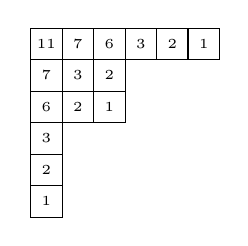
\begin{tikzpicture}
  \draw (0.00, 0.00) rectangle (0.40, -0.40);
  \node[font=\tiny] at (0.20, -0.20) {11};
  \draw (0.40, 0.00) rectangle (0.80, -0.40);
  \node[font=\tiny] at (0.60, -0.20) {7};
  \draw (0.80, 0.00) rectangle (1.20, -0.40);
  \node[font=\tiny] at (1.00, -0.20) {6};
  \draw (1.20, 0.00) rectangle (1.60, -0.40);
  \node[font=\tiny] at (1.40, -0.20) {3};
  \draw (1.60, 0.00) rectangle (2.00, -0.40);
  \node[font=\tiny] at (1.80, -0.20) {2};
  \draw (2.00, 0.00) rectangle (2.40, -0.40);
  \node[font=\tiny] at (2.20, -0.20) {1};
  \draw (0.00, -0.40) rectangle (0.40, -0.80);
  \node[font=\tiny] at (0.20, -0.60) {7};
  \draw (0.40, -0.40) rectangle (0.80, -0.80);
  \node[font=\tiny] at (0.60, -0.60) {3};
  \draw (0.80, -0.40) rectangle (1.20, -0.80);
  \node[font=\tiny] at (1.00, -0.60) {2};
  \draw (0.00, -0.80) rectangle (0.40, -1.20);
  \node[font=\tiny] at (0.20, -1.00) {6};
  \draw (0.40, -0.80) rectangle (0.80, -1.20);
  \node[font=\tiny] at (0.60, -1.00) {2};
  \draw (0.80, -0.80) rectangle (1.20, -1.20);
  \node[font=\tiny] at (1.00, -1.00) {1};
  \draw (0.00, -1.20) rectangle (0.40, -1.60);
  \node[font=\tiny] at (0.20, -1.40) {3};
  \draw (0.00, -1.60) rectangle (0.40, -2.00);
  \node[font=\tiny] at (0.20, -1.80) {2};
  \draw (0.00, -2.00) rectangle (0.40, -2.40);
  \node[font=\tiny] at (0.20, -2.20) {1};
\end{tikzpicture}
\end{minipage}
\vspace{1cm}
\noindent \newline\begin{minipage}{0.48\textwidth}
\subsubsection*{Gap Poset}
\centering
\begin{tikzpicture}
  \node[minimum size=0.3cm] (1) at (0.00,-3.20) {1};
  \node[minimum size=0.3cm] (2) at (1.60,-3.20) {2};
  \node[minimum size=0.3cm] (3) at (3.20,-3.20) {3};
  \node[minimum size=0.3cm] (6) at (0.00,-1.60) {6};
  \node[minimum size=0.3cm] (7) at (1.60,-1.60) {7};
  \node[draw, rectangle, minimum size=0.3cm] (11) at (0.00,0.00) {11};
  % Draw the cover relations
  \draw (11) -- (7);
  \draw (6) -- (2);
  \draw (6) -- (1);
  \draw (11) -- (6);
  \draw (7) -- (3);
  \draw (7) -- (2);
\end{tikzpicture}
\end{minipage}%
\hfill\begin{minipage}{0.48\textwidth}
\subsubsection*{Void Poset}
\centering
\end{minipage}
\newpage\subsection{[5, 7, 9, 11]}
\noindent\begin{minipage}{0.6\textwidth}
\subsubsection*{Invariants}
\centering
\begin{tabular}{|c|c|c|c|c|c|c|}
\toprule
g & F & m & ewt & t & \(|M|\) & \(|\lambda|\) \\
\midrule
7 & 13 & 5 & 7 & 1 & 0 & 16 \\
\bottomrule
\end{tabular}
\end{minipage}%
\begin{minipage}{0.4\textwidth}
\subsubsection*{Partition}
\centering
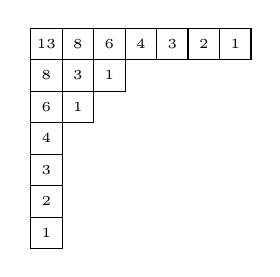
\begin{tikzpicture}
  \draw (0.00, 0.00) rectangle (0.40, -0.40);
  \node[font=\tiny] at (0.20, -0.20) {13};
  \draw (0.40, 0.00) rectangle (0.80, -0.40);
  \node[font=\tiny] at (0.60, -0.20) {8};
  \draw (0.80, 0.00) rectangle (1.20, -0.40);
  \node[font=\tiny] at (1.00, -0.20) {6};
  \draw (1.20, 0.00) rectangle (1.60, -0.40);
  \node[font=\tiny] at (1.40, -0.20) {4};
  \draw (1.60, 0.00) rectangle (2.00, -0.40);
  \node[font=\tiny] at (1.80, -0.20) {3};
  \draw (2.00, 0.00) rectangle (2.40, -0.40);
  \node[font=\tiny] at (2.20, -0.20) {2};
  \draw (2.40, 0.00) rectangle (2.80, -0.40);
  \node[font=\tiny] at (2.60, -0.20) {1};
  \draw (0.00, -0.40) rectangle (0.40, -0.80);
  \node[font=\tiny] at (0.20, -0.60) {8};
  \draw (0.40, -0.40) rectangle (0.80, -0.80);
  \node[font=\tiny] at (0.60, -0.60) {3};
  \draw (0.80, -0.40) rectangle (1.20, -0.80);
  \node[font=\tiny] at (1.00, -0.60) {1};
  \draw (0.00, -0.80) rectangle (0.40, -1.20);
  \node[font=\tiny] at (0.20, -1.00) {6};
  \draw (0.40, -0.80) rectangle (0.80, -1.20);
  \node[font=\tiny] at (0.60, -1.00) {1};
  \draw (0.00, -1.20) rectangle (0.40, -1.60);
  \node[font=\tiny] at (0.20, -1.40) {4};
  \draw (0.00, -1.60) rectangle (0.40, -2.00);
  \node[font=\tiny] at (0.20, -1.80) {3};
  \draw (0.00, -2.00) rectangle (0.40, -2.40);
  \node[font=\tiny] at (0.20, -2.20) {2};
  \draw (0.00, -2.40) rectangle (0.40, -2.80);
  \node[font=\tiny] at (0.20, -2.60) {1};
\end{tikzpicture}
\end{minipage}
\vspace{1cm}
\noindent \newline\begin{minipage}{0.48\textwidth}
\subsubsection*{Gap Poset}
\centering
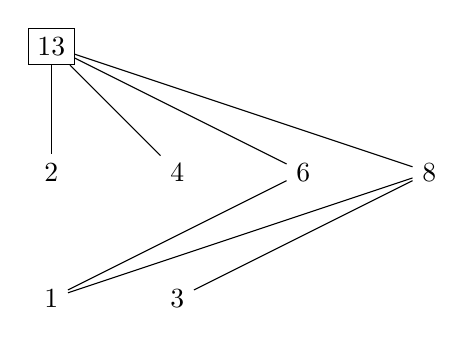
\begin{tikzpicture}
  \node[minimum size=0.3cm] (1) at (0.00,-3.20) {1};
  \node[minimum size=0.3cm] (3) at (1.60,-3.20) {3};
  \node[minimum size=0.3cm] (2) at (0.00,-1.60) {2};
  \node[minimum size=0.3cm] (4) at (1.60,-1.60) {4};
  \node[minimum size=0.3cm] (6) at (3.20,-1.60) {6};
  \node[minimum size=0.3cm] (8) at (4.80,-1.60) {8};
  \node[draw, rectangle, minimum size=0.3cm] (13) at (0.00,0.00) {13};
  % Draw the cover relations
  \draw (13) -- (8);
  \draw (13) -- (4);
  \draw (8) -- (1);
  \draw (6) -- (1);
  \draw (8) -- (3);
  \draw (13) -- (6);
  \draw (13) -- (2);
\end{tikzpicture}
\end{minipage}%
\hfill\begin{minipage}{0.48\textwidth}
\subsubsection*{Void Poset}
\centering
\end{minipage}
\newpage\subsection{[5, 7, 8]}
\noindent\begin{minipage}{0.6\textwidth}
\subsubsection*{Invariants}
\centering
\begin{tabular}{|c|c|c|c|c|c|c|}
\toprule
g & F & m & ewt & t & \(|M|\) & \(|\lambda|\) \\
\midrule
7 & 11 & 5 & 7 & 2 & 2 & 15 \\
\bottomrule
\end{tabular}
\end{minipage}%
\begin{minipage}{0.4\textwidth}
\subsubsection*{Partition}
\centering
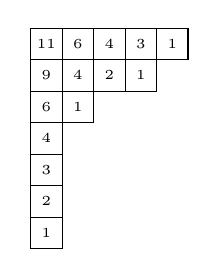
\begin{tikzpicture}
  \draw (0.00, 0.00) rectangle (0.40, -0.40);
  \node[font=\tiny] at (0.20, -0.20) {11};
  \draw (0.40, 0.00) rectangle (0.80, -0.40);
  \node[font=\tiny] at (0.60, -0.20) {6};
  \draw (0.80, 0.00) rectangle (1.20, -0.40);
  \node[font=\tiny] at (1.00, -0.20) {4};
  \draw (1.20, 0.00) rectangle (1.60, -0.40);
  \node[font=\tiny] at (1.40, -0.20) {3};
  \draw (1.60, 0.00) rectangle (2.00, -0.40);
  \node[font=\tiny] at (1.80, -0.20) {1};
  \draw (0.00, -0.40) rectangle (0.40, -0.80);
  \node[font=\tiny] at (0.20, -0.60) {9};
  \draw (0.40, -0.40) rectangle (0.80, -0.80);
  \node[font=\tiny] at (0.60, -0.60) {4};
  \draw (0.80, -0.40) rectangle (1.20, -0.80);
  \node[font=\tiny] at (1.00, -0.60) {2};
  \draw (1.20, -0.40) rectangle (1.60, -0.80);
  \node[font=\tiny] at (1.40, -0.60) {1};
  \draw (0.00, -0.80) rectangle (0.40, -1.20);
  \node[font=\tiny] at (0.20, -1.00) {6};
  \draw (0.40, -0.80) rectangle (0.80, -1.20);
  \node[font=\tiny] at (0.60, -1.00) {1};
  \draw (0.00, -1.20) rectangle (0.40, -1.60);
  \node[font=\tiny] at (0.20, -1.40) {4};
  \draw (0.00, -1.60) rectangle (0.40, -2.00);
  \node[font=\tiny] at (0.20, -1.80) {3};
  \draw (0.00, -2.00) rectangle (0.40, -2.40);
  \node[font=\tiny] at (0.20, -2.20) {2};
  \draw (0.00, -2.40) rectangle (0.40, -2.80);
  \node[font=\tiny] at (0.20, -2.60) {1};
\end{tikzpicture}
\end{minipage}
\vspace{1cm}
\noindent \newline\begin{minipage}{0.48\textwidth}
\subsubsection*{Gap Poset}
\centering
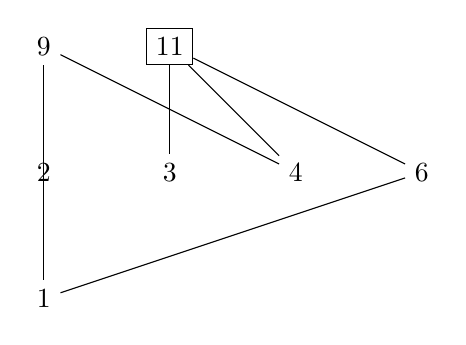
\begin{tikzpicture}
  \node[minimum size=0.3cm] (1) at (0.00,-3.20) {1};
  \node[minimum size=0.3cm] (2) at (0.00,-1.60) {2};
  \node[minimum size=0.3cm] (3) at (1.60,-1.60) {3};
  \node[minimum size=0.3cm] (4) at (3.20,-1.60) {4};
  \node[minimum size=0.3cm] (6) at (4.80,-1.60) {6};
  \node[minimum size=0.3cm] (9) at (0.00,0.00) {9};
  \node[draw, rectangle, minimum size=0.3cm] (11) at (1.60,0.00) {11};
  % Draw the cover relations
  \draw (6) -- (1);
  \draw (11) -- (3);
  \draw (9) -- (2);
  \draw (11) -- (6);
  \draw (9) -- (1);
  \draw (11) -- (4);
  \draw (9) -- (4);
\end{tikzpicture}
\end{minipage}%
\hfill\begin{minipage}{0.48\textwidth}
\subsubsection*{Void Poset}
\centering
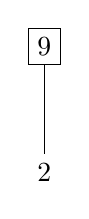
\begin{tikzpicture}
  \node[draw, rectangle, minimum size=0.3cm] (9) at (0.00,0.00) {9};
  \node[minimum size=0.3cm] (2) at (0.00,-1.60) {2};
  % Draw the cover relations
  \draw (9) -- (2);
\end{tikzpicture}
\end{minipage}
\newpage\subsection{[5, 6, 9]}
\noindent\begin{minipage}{0.6\textwidth}
\subsubsection*{Invariants}
\centering
\begin{tabular}{|c|c|c|c|c|c|c|}
\toprule
g & F & m & ewt & t & \(|M|\) & \(|\lambda|\) \\
\midrule
7 & 13 & 5 & 7 & 1 & 0 & 17 \\
\bottomrule
\end{tabular}
\end{minipage}%
\begin{minipage}{0.4\textwidth}
\subsubsection*{Partition}
\centering
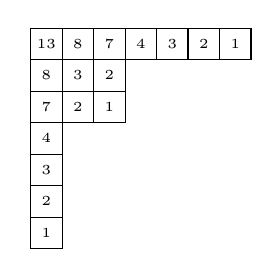
\begin{tikzpicture}
  \draw (0.00, 0.00) rectangle (0.40, -0.40);
  \node[font=\tiny] at (0.20, -0.20) {13};
  \draw (0.40, 0.00) rectangle (0.80, -0.40);
  \node[font=\tiny] at (0.60, -0.20) {8};
  \draw (0.80, 0.00) rectangle (1.20, -0.40);
  \node[font=\tiny] at (1.00, -0.20) {7};
  \draw (1.20, 0.00) rectangle (1.60, -0.40);
  \node[font=\tiny] at (1.40, -0.20) {4};
  \draw (1.60, 0.00) rectangle (2.00, -0.40);
  \node[font=\tiny] at (1.80, -0.20) {3};
  \draw (2.00, 0.00) rectangle (2.40, -0.40);
  \node[font=\tiny] at (2.20, -0.20) {2};
  \draw (2.40, 0.00) rectangle (2.80, -0.40);
  \node[font=\tiny] at (2.60, -0.20) {1};
  \draw (0.00, -0.40) rectangle (0.40, -0.80);
  \node[font=\tiny] at (0.20, -0.60) {8};
  \draw (0.40, -0.40) rectangle (0.80, -0.80);
  \node[font=\tiny] at (0.60, -0.60) {3};
  \draw (0.80, -0.40) rectangle (1.20, -0.80);
  \node[font=\tiny] at (1.00, -0.60) {2};
  \draw (0.00, -0.80) rectangle (0.40, -1.20);
  \node[font=\tiny] at (0.20, -1.00) {7};
  \draw (0.40, -0.80) rectangle (0.80, -1.20);
  \node[font=\tiny] at (0.60, -1.00) {2};
  \draw (0.80, -0.80) rectangle (1.20, -1.20);
  \node[font=\tiny] at (1.00, -1.00) {1};
  \draw (0.00, -1.20) rectangle (0.40, -1.60);
  \node[font=\tiny] at (0.20, -1.40) {4};
  \draw (0.00, -1.60) rectangle (0.40, -2.00);
  \node[font=\tiny] at (0.20, -1.80) {3};
  \draw (0.00, -2.00) rectangle (0.40, -2.40);
  \node[font=\tiny] at (0.20, -2.20) {2};
  \draw (0.00, -2.40) rectangle (0.40, -2.80);
  \node[font=\tiny] at (0.20, -2.60) {1};
\end{tikzpicture}
\end{minipage}
\vspace{1cm}
\noindent \newline\begin{minipage}{0.48\textwidth}
\subsubsection*{Gap Poset}
\centering
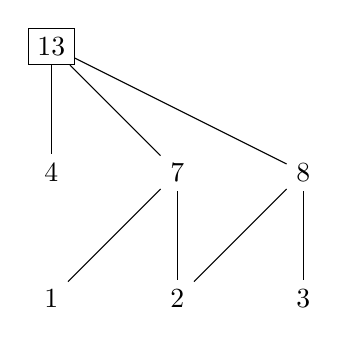
\begin{tikzpicture}
  \node[minimum size=0.3cm] (1) at (0.00,-3.20) {1};
  \node[minimum size=0.3cm] (2) at (1.60,-3.20) {2};
  \node[minimum size=0.3cm] (3) at (3.20,-3.20) {3};
  \node[minimum size=0.3cm] (4) at (0.00,-1.60) {4};
  \node[minimum size=0.3cm] (7) at (1.60,-1.60) {7};
  \node[minimum size=0.3cm] (8) at (3.20,-1.60) {8};
  \node[draw, rectangle, minimum size=0.3cm] (13) at (0.00,0.00) {13};
  % Draw the cover relations
  \draw (13) -- (8);
  \draw (13) -- (4);
  \draw (7) -- (1);
  \draw (13) -- (7);
  \draw (8) -- (3);
  \draw (7) -- (2);
  \draw (8) -- (2);
\end{tikzpicture}
\end{minipage}%
\hfill\begin{minipage}{0.48\textwidth}
\subsubsection*{Void Poset}
\centering
\end{minipage}
\newpage\subsection{[4, 6, 13, 15]}
\noindent\begin{minipage}{0.6\textwidth}
\subsubsection*{Invariants}
\centering
\begin{tabular}{|c|c|c|c|c|c|c|}
\toprule
g & F & m & ewt & t & \(|M|\) & \(|\lambda|\) \\
\midrule
7 & 11 & 4 & 7 & 3 & 2 & 17 \\
\bottomrule
\end{tabular}
\end{minipage}%
\begin{minipage}{0.4\textwidth}
\subsubsection*{Partition}
\centering
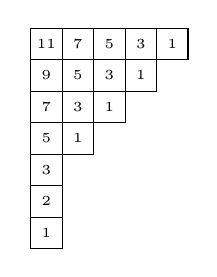
\begin{tikzpicture}
  \draw (0.00, 0.00) rectangle (0.40, -0.40);
  \node[font=\tiny] at (0.20, -0.20) {11};
  \draw (0.40, 0.00) rectangle (0.80, -0.40);
  \node[font=\tiny] at (0.60, -0.20) {7};
  \draw (0.80, 0.00) rectangle (1.20, -0.40);
  \node[font=\tiny] at (1.00, -0.20) {5};
  \draw (1.20, 0.00) rectangle (1.60, -0.40);
  \node[font=\tiny] at (1.40, -0.20) {3};
  \draw (1.60, 0.00) rectangle (2.00, -0.40);
  \node[font=\tiny] at (1.80, -0.20) {1};
  \draw (0.00, -0.40) rectangle (0.40, -0.80);
  \node[font=\tiny] at (0.20, -0.60) {9};
  \draw (0.40, -0.40) rectangle (0.80, -0.80);
  \node[font=\tiny] at (0.60, -0.60) {5};
  \draw (0.80, -0.40) rectangle (1.20, -0.80);
  \node[font=\tiny] at (1.00, -0.60) {3};
  \draw (1.20, -0.40) rectangle (1.60, -0.80);
  \node[font=\tiny] at (1.40, -0.60) {1};
  \draw (0.00, -0.80) rectangle (0.40, -1.20);
  \node[font=\tiny] at (0.20, -1.00) {7};
  \draw (0.40, -0.80) rectangle (0.80, -1.20);
  \node[font=\tiny] at (0.60, -1.00) {3};
  \draw (0.80, -0.80) rectangle (1.20, -1.20);
  \node[font=\tiny] at (1.00, -1.00) {1};
  \draw (0.00, -1.20) rectangle (0.40, -1.60);
  \node[font=\tiny] at (0.20, -1.40) {5};
  \draw (0.40, -1.20) rectangle (0.80, -1.60);
  \node[font=\tiny] at (0.60, -1.40) {1};
  \draw (0.00, -1.60) rectangle (0.40, -2.00);
  \node[font=\tiny] at (0.20, -1.80) {3};
  \draw (0.00, -2.00) rectangle (0.40, -2.40);
  \node[font=\tiny] at (0.20, -2.20) {2};
  \draw (0.00, -2.40) rectangle (0.40, -2.80);
  \node[font=\tiny] at (0.20, -2.60) {1};
\end{tikzpicture}
\end{minipage}
\vspace{1cm}
\noindent \newline\begin{minipage}{0.48\textwidth}
\subsubsection*{Gap Poset}
\centering
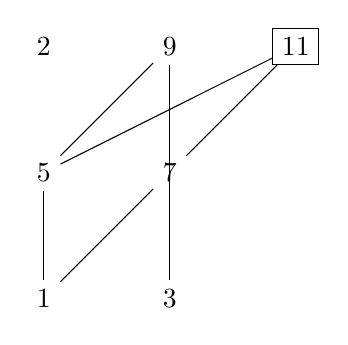
\begin{tikzpicture}
  \node[minimum size=0.3cm] (1) at (0.00,-3.20) {1};
  \node[minimum size=0.3cm] (3) at (1.60,-3.20) {3};
  \node[minimum size=0.3cm] (2) at (0.00,0.00) {2};
  \node[minimum size=0.3cm] (9) at (1.60,0.00) {9};
  \node[draw, rectangle, minimum size=0.3cm] (11) at (3.20,0.00) {11};
  \node[minimum size=0.3cm] (5) at (0.00,-1.60) {5};
  \node[minimum size=0.3cm] (7) at (1.60,-1.60) {7};
  % Draw the cover relations
  \draw (11) -- (7);
  \draw (7) -- (1);
  \draw (9) -- (3);
  \draw (5) -- (1);
  \draw (7) -- (3);
  \draw (9) -- (5);
  \draw (11) -- (5);
\end{tikzpicture}
\end{minipage}%
\hfill\begin{minipage}{0.48\textwidth}
\subsubsection*{Void Poset}
\centering
\begin{tikzpicture}
  \node[draw, rectangle, minimum size=0.3cm] (9) at (0.00,0.00) {9};
  \node[minimum size=0.3cm] (2) at (1.60,0.00) {2};
\end{tikzpicture}
\end{minipage}
\newpage\subsection{[6, 8, 9, 10]}
\noindent\begin{minipage}{0.6\textwidth}
\subsubsection*{Invariants}
\centering
\begin{tabular}{|c|c|c|c|c|c|c|}
\toprule
g & F & m & ewt & t & \(|M|\) & \(|\lambda|\) \\
\midrule
8 & 13 & 6 & 9 & 2 & 2 & 18 \\
\bottomrule
\end{tabular}
\end{minipage}%
\begin{minipage}{0.4\textwidth}
\subsubsection*{Partition}
\centering
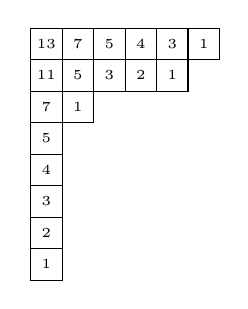
\begin{tikzpicture}
  \draw (0.00, 0.00) rectangle (0.40, -0.40);
  \node[font=\tiny] at (0.20, -0.20) {13};
  \draw (0.40, 0.00) rectangle (0.80, -0.40);
  \node[font=\tiny] at (0.60, -0.20) {7};
  \draw (0.80, 0.00) rectangle (1.20, -0.40);
  \node[font=\tiny] at (1.00, -0.20) {5};
  \draw (1.20, 0.00) rectangle (1.60, -0.40);
  \node[font=\tiny] at (1.40, -0.20) {4};
  \draw (1.60, 0.00) rectangle (2.00, -0.40);
  \node[font=\tiny] at (1.80, -0.20) {3};
  \draw (2.00, 0.00) rectangle (2.40, -0.40);
  \node[font=\tiny] at (2.20, -0.20) {1};
  \draw (0.00, -0.40) rectangle (0.40, -0.80);
  \node[font=\tiny] at (0.20, -0.60) {11};
  \draw (0.40, -0.40) rectangle (0.80, -0.80);
  \node[font=\tiny] at (0.60, -0.60) {5};
  \draw (0.80, -0.40) rectangle (1.20, -0.80);
  \node[font=\tiny] at (1.00, -0.60) {3};
  \draw (1.20, -0.40) rectangle (1.60, -0.80);
  \node[font=\tiny] at (1.40, -0.60) {2};
  \draw (1.60, -0.40) rectangle (2.00, -0.80);
  \node[font=\tiny] at (1.80, -0.60) {1};
  \draw (0.00, -0.80) rectangle (0.40, -1.20);
  \node[font=\tiny] at (0.20, -1.00) {7};
  \draw (0.40, -0.80) rectangle (0.80, -1.20);
  \node[font=\tiny] at (0.60, -1.00) {1};
  \draw (0.00, -1.20) rectangle (0.40, -1.60);
  \node[font=\tiny] at (0.20, -1.40) {5};
  \draw (0.00, -1.60) rectangle (0.40, -2.00);
  \node[font=\tiny] at (0.20, -1.80) {4};
  \draw (0.00, -2.00) rectangle (0.40, -2.40);
  \node[font=\tiny] at (0.20, -2.20) {3};
  \draw (0.00, -2.40) rectangle (0.40, -2.80);
  \node[font=\tiny] at (0.20, -2.60) {2};
  \draw (0.00, -2.80) rectangle (0.40, -3.20);
  \node[font=\tiny] at (0.20, -3.00) {1};
\end{tikzpicture}
\end{minipage}
\vspace{1cm}
\noindent \newline\begin{minipage}{0.48\textwidth}
\subsubsection*{Gap Poset}
\centering
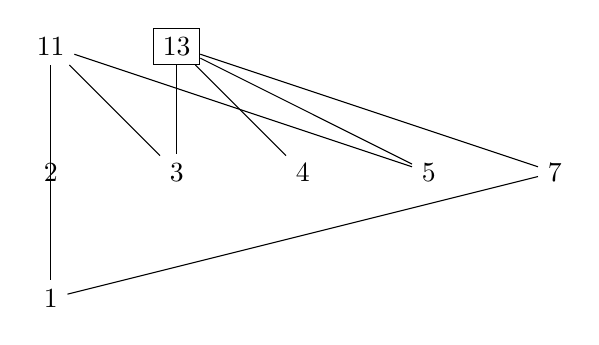
\begin{tikzpicture}
  \node[minimum size=0.3cm] (1) at (0.00,-3.20) {1};
  \node[minimum size=0.3cm] (2) at (0.00,-1.60) {2};
  \node[minimum size=0.3cm] (3) at (1.60,-1.60) {3};
  \node[minimum size=0.3cm] (4) at (3.20,-1.60) {4};
  \node[minimum size=0.3cm] (5) at (4.80,-1.60) {5};
  \node[minimum size=0.3cm] (7) at (6.40,-1.60) {7};
  \node[minimum size=0.3cm] (11) at (0.00,0.00) {11};
  \node[draw, rectangle, minimum size=0.3cm] (13) at (1.60,0.00) {13};
  % Draw the cover relations
  \draw (11) -- (1);
  \draw (13) -- (4);
  \draw (7) -- (1);
  \draw (13) -- (7);
  \draw (11) -- (3);
  \draw (13) -- (3);
  \draw (11) -- (2);
  \draw (11) -- (5);
  \draw (13) -- (5);
\end{tikzpicture}
\end{minipage}%
\hfill\begin{minipage}{0.48\textwidth}
\subsubsection*{Void Poset}
\centering
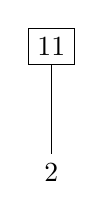
\begin{tikzpicture}
  \node[minimum size=0.3cm] (2) at (0.00,-1.60) {2};
  \node[draw, rectangle, minimum size=0.3cm] (11) at (0.00,0.00) {11};
  % Draw the cover relations
  \draw (11) -- (2);
\end{tikzpicture}
\end{minipage}
\newpage\subsection{[5, 7, 9]}
\noindent\begin{minipage}{0.6\textwidth}
\subsubsection*{Invariants}
\centering
\begin{tabular}{|c|c|c|c|c|c|c|}
\toprule
g & F & m & ewt & t & \(|M|\) & \(|\lambda|\) \\
\midrule
8 & 13 & 5 & 9 & 2 & 2 & 20 \\
\bottomrule
\end{tabular}
\end{minipage}%
\begin{minipage}{0.4\textwidth}
\subsubsection*{Partition}
\centering
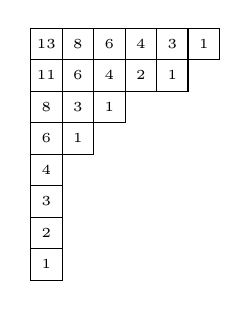
\begin{tikzpicture}
  \draw (0.00, 0.00) rectangle (0.40, -0.40);
  \node[font=\tiny] at (0.20, -0.20) {13};
  \draw (0.40, 0.00) rectangle (0.80, -0.40);
  \node[font=\tiny] at (0.60, -0.20) {8};
  \draw (0.80, 0.00) rectangle (1.20, -0.40);
  \node[font=\tiny] at (1.00, -0.20) {6};
  \draw (1.20, 0.00) rectangle (1.60, -0.40);
  \node[font=\tiny] at (1.40, -0.20) {4};
  \draw (1.60, 0.00) rectangle (2.00, -0.40);
  \node[font=\tiny] at (1.80, -0.20) {3};
  \draw (2.00, 0.00) rectangle (2.40, -0.40);
  \node[font=\tiny] at (2.20, -0.20) {1};
  \draw (0.00, -0.40) rectangle (0.40, -0.80);
  \node[font=\tiny] at (0.20, -0.60) {11};
  \draw (0.40, -0.40) rectangle (0.80, -0.80);
  \node[font=\tiny] at (0.60, -0.60) {6};
  \draw (0.80, -0.40) rectangle (1.20, -0.80);
  \node[font=\tiny] at (1.00, -0.60) {4};
  \draw (1.20, -0.40) rectangle (1.60, -0.80);
  \node[font=\tiny] at (1.40, -0.60) {2};
  \draw (1.60, -0.40) rectangle (2.00, -0.80);
  \node[font=\tiny] at (1.80, -0.60) {1};
  \draw (0.00, -0.80) rectangle (0.40, -1.20);
  \node[font=\tiny] at (0.20, -1.00) {8};
  \draw (0.40, -0.80) rectangle (0.80, -1.20);
  \node[font=\tiny] at (0.60, -1.00) {3};
  \draw (0.80, -0.80) rectangle (1.20, -1.20);
  \node[font=\tiny] at (1.00, -1.00) {1};
  \draw (0.00, -1.20) rectangle (0.40, -1.60);
  \node[font=\tiny] at (0.20, -1.40) {6};
  \draw (0.40, -1.20) rectangle (0.80, -1.60);
  \node[font=\tiny] at (0.60, -1.40) {1};
  \draw (0.00, -1.60) rectangle (0.40, -2.00);
  \node[font=\tiny] at (0.20, -1.80) {4};
  \draw (0.00, -2.00) rectangle (0.40, -2.40);
  \node[font=\tiny] at (0.20, -2.20) {3};
  \draw (0.00, -2.40) rectangle (0.40, -2.80);
  \node[font=\tiny] at (0.20, -2.60) {2};
  \draw (0.00, -2.80) rectangle (0.40, -3.20);
  \node[font=\tiny] at (0.20, -3.00) {1};
\end{tikzpicture}
\end{minipage}
\vspace{1cm}
\noindent \newline\begin{minipage}{0.48\textwidth}
\subsubsection*{Gap Poset}
\centering
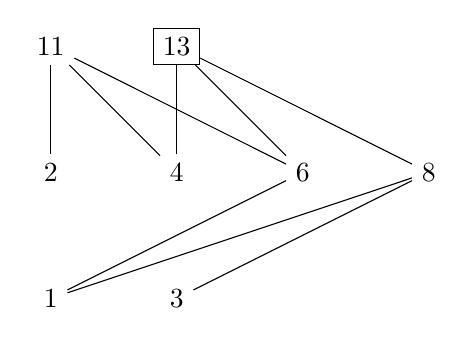
\begin{tikzpicture}
  \node[minimum size=0.3cm] (1) at (0.00,-3.20) {1};
  \node[minimum size=0.3cm] (3) at (1.60,-3.20) {3};
  \node[minimum size=0.3cm] (2) at (0.00,-1.60) {2};
  \node[minimum size=0.3cm] (4) at (1.60,-1.60) {4};
  \node[minimum size=0.3cm] (6) at (3.20,-1.60) {6};
  \node[minimum size=0.3cm] (8) at (4.80,-1.60) {8};
  \node[minimum size=0.3cm] (11) at (0.00,0.00) {11};
  \node[draw, rectangle, minimum size=0.3cm] (13) at (1.60,0.00) {13};
  % Draw the cover relations
  \draw (13) -- (8);
  \draw (13) -- (4);
  \draw (8) -- (1);
  \draw (6) -- (1);
  \draw (11) -- (6);
  \draw (11) -- (2);
  \draw (8) -- (3);
  \draw (13) -- (6);
  \draw (11) -- (4);
\end{tikzpicture}
\end{minipage}%
\hfill\begin{minipage}{0.48\textwidth}
\subsubsection*{Void Poset}
\centering
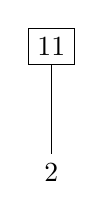
\begin{tikzpicture}
  \node[minimum size=0.3cm] (2) at (0.00,-1.60) {2};
  \node[draw, rectangle, minimum size=0.3cm] (11) at (0.00,0.00) {11};
  % Draw the cover relations
  \draw (11) -- (2);
\end{tikzpicture}
\end{minipage}
\newpage\subsection{[5, 6, 13]}
\noindent\begin{minipage}{0.6\textwidth}
\subsubsection*{Invariants}
\centering
\begin{tabular}{|c|c|c|c|c|c|c|}
\toprule
g & F & m & ewt & t & \(|M|\) & \(|\lambda|\) \\
\midrule
8 & 14 & 5 & 9 & 2 & 1 & 20 \\
\bottomrule
\end{tabular}
\end{minipage}%
\begin{minipage}{0.4\textwidth}
\subsubsection*{Partition}
\centering
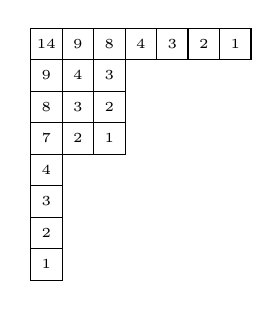
\begin{tikzpicture}
  \draw (0.00, 0.00) rectangle (0.40, -0.40);
  \node[font=\tiny] at (0.20, -0.20) {14};
  \draw (0.40, 0.00) rectangle (0.80, -0.40);
  \node[font=\tiny] at (0.60, -0.20) {9};
  \draw (0.80, 0.00) rectangle (1.20, -0.40);
  \node[font=\tiny] at (1.00, -0.20) {8};
  \draw (1.20, 0.00) rectangle (1.60, -0.40);
  \node[font=\tiny] at (1.40, -0.20) {4};
  \draw (1.60, 0.00) rectangle (2.00, -0.40);
  \node[font=\tiny] at (1.80, -0.20) {3};
  \draw (2.00, 0.00) rectangle (2.40, -0.40);
  \node[font=\tiny] at (2.20, -0.20) {2};
  \draw (2.40, 0.00) rectangle (2.80, -0.40);
  \node[font=\tiny] at (2.60, -0.20) {1};
  \draw (0.00, -0.40) rectangle (0.40, -0.80);
  \node[font=\tiny] at (0.20, -0.60) {9};
  \draw (0.40, -0.40) rectangle (0.80, -0.80);
  \node[font=\tiny] at (0.60, -0.60) {4};
  \draw (0.80, -0.40) rectangle (1.20, -0.80);
  \node[font=\tiny] at (1.00, -0.60) {3};
  \draw (0.00, -0.80) rectangle (0.40, -1.20);
  \node[font=\tiny] at (0.20, -1.00) {8};
  \draw (0.40, -0.80) rectangle (0.80, -1.20);
  \node[font=\tiny] at (0.60, -1.00) {3};
  \draw (0.80, -0.80) rectangle (1.20, -1.20);
  \node[font=\tiny] at (1.00, -1.00) {2};
  \draw (0.00, -1.20) rectangle (0.40, -1.60);
  \node[font=\tiny] at (0.20, -1.40) {7};
  \draw (0.40, -1.20) rectangle (0.80, -1.60);
  \node[font=\tiny] at (0.60, -1.40) {2};
  \draw (0.80, -1.20) rectangle (1.20, -1.60);
  \node[font=\tiny] at (1.00, -1.40) {1};
  \draw (0.00, -1.60) rectangle (0.40, -2.00);
  \node[font=\tiny] at (0.20, -1.80) {4};
  \draw (0.00, -2.00) rectangle (0.40, -2.40);
  \node[font=\tiny] at (0.20, -2.20) {3};
  \draw (0.00, -2.40) rectangle (0.40, -2.80);
  \node[font=\tiny] at (0.20, -2.60) {2};
  \draw (0.00, -2.80) rectangle (0.40, -3.20);
  \node[font=\tiny] at (0.20, -3.00) {1};
\end{tikzpicture}
\end{minipage}
\vspace{1cm}
\noindent \newline\begin{minipage}{0.48\textwidth}
\subsubsection*{Gap Poset}
\centering
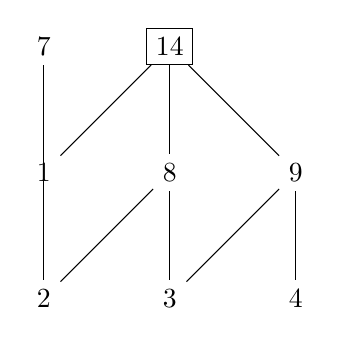
\begin{tikzpicture}
  \node[minimum size=0.3cm] (1) at (0.00,-1.60) {1};
  \node[minimum size=0.3cm] (8) at (1.60,-1.60) {8};
  \node[minimum size=0.3cm] (9) at (3.20,-1.60) {9};
  \node[minimum size=0.3cm] (2) at (0.00,-3.20) {2};
  \node[minimum size=0.3cm] (3) at (1.60,-3.20) {3};
  \node[minimum size=0.3cm] (4) at (3.20,-3.20) {4};
  \node[minimum size=0.3cm] (7) at (0.00,0.00) {7};
  \node[draw, rectangle, minimum size=0.3cm] (14) at (1.60,0.00) {14};
  % Draw the cover relations
  \draw (14) -- (8);
  \draw (7) -- (1);
  \draw (9) -- (3);
  \draw (14) -- (1);
  \draw (8) -- (3);
  \draw (14) -- (9);
  \draw (7) -- (2);
  \draw (8) -- (2);
  \draw (9) -- (4);
\end{tikzpicture}
\end{minipage}%
\hfill\begin{minipage}{0.48\textwidth}
\subsubsection*{Void Poset}
\centering

\begin{tikzpicture}
  \node[draw, rectangle, minimum size=0.3cm] (7) at (0.00,0.00) {7};
\end{tikzpicture}
\end{minipage}
\newpage\subsection{[6, 7, 8]}
\noindent\begin{minipage}{0.6\textwidth}
\subsubsection*{Invariants}
\centering
\begin{tabular}{|c|c|c|c|c|c|c|}
\toprule
g & F & m & ewt & t & \(|M|\) & \(|\lambda|\) \\
\midrule
9 & 17 & 6 & 12 & 1 & 0 & 26 \\
\bottomrule
\end{tabular}
\end{minipage}%
\begin{minipage}{0.4\textwidth}
\subsubsection*{Partition}
\centering
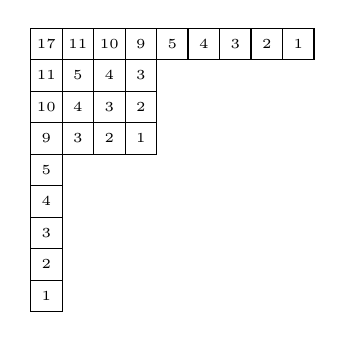
\begin{tikzpicture}
  \draw (0.00, 0.00) rectangle (0.40, -0.40);
  \node[font=\tiny] at (0.20, -0.20) {17};
  \draw (0.40, 0.00) rectangle (0.80, -0.40);
  \node[font=\tiny] at (0.60, -0.20) {11};
  \draw (0.80, 0.00) rectangle (1.20, -0.40);
  \node[font=\tiny] at (1.00, -0.20) {10};
  \draw (1.20, 0.00) rectangle (1.60, -0.40);
  \node[font=\tiny] at (1.40, -0.20) {9};
  \draw (1.60, 0.00) rectangle (2.00, -0.40);
  \node[font=\tiny] at (1.80, -0.20) {5};
  \draw (2.00, 0.00) rectangle (2.40, -0.40);
  \node[font=\tiny] at (2.20, -0.20) {4};
  \draw (2.40, 0.00) rectangle (2.80, -0.40);
  \node[font=\tiny] at (2.60, -0.20) {3};
  \draw (2.80, 0.00) rectangle (3.20, -0.40);
  \node[font=\tiny] at (3.00, -0.20) {2};
  \draw (3.20, 0.00) rectangle (3.60, -0.40);
  \node[font=\tiny] at (3.40, -0.20) {1};
  \draw (0.00, -0.40) rectangle (0.40, -0.80);
  \node[font=\tiny] at (0.20, -0.60) {11};
  \draw (0.40, -0.40) rectangle (0.80, -0.80);
  \node[font=\tiny] at (0.60, -0.60) {5};
  \draw (0.80, -0.40) rectangle (1.20, -0.80);
  \node[font=\tiny] at (1.00, -0.60) {4};
  \draw (1.20, -0.40) rectangle (1.60, -0.80);
  \node[font=\tiny] at (1.40, -0.60) {3};
  \draw (0.00, -0.80) rectangle (0.40, -1.20);
  \node[font=\tiny] at (0.20, -1.00) {10};
  \draw (0.40, -0.80) rectangle (0.80, -1.20);
  \node[font=\tiny] at (0.60, -1.00) {4};
  \draw (0.80, -0.80) rectangle (1.20, -1.20);
  \node[font=\tiny] at (1.00, -1.00) {3};
  \draw (1.20, -0.80) rectangle (1.60, -1.20);
  \node[font=\tiny] at (1.40, -1.00) {2};
  \draw (0.00, -1.20) rectangle (0.40, -1.60);
  \node[font=\tiny] at (0.20, -1.40) {9};
  \draw (0.40, -1.20) rectangle (0.80, -1.60);
  \node[font=\tiny] at (0.60, -1.40) {3};
  \draw (0.80, -1.20) rectangle (1.20, -1.60);
  \node[font=\tiny] at (1.00, -1.40) {2};
  \draw (1.20, -1.20) rectangle (1.60, -1.60);
  \node[font=\tiny] at (1.40, -1.40) {1};
  \draw (0.00, -1.60) rectangle (0.40, -2.00);
  \node[font=\tiny] at (0.20, -1.80) {5};
  \draw (0.00, -2.00) rectangle (0.40, -2.40);
  \node[font=\tiny] at (0.20, -2.20) {4};
  \draw (0.00, -2.40) rectangle (0.40, -2.80);
  \node[font=\tiny] at (0.20, -2.60) {3};
  \draw (0.00, -2.80) rectangle (0.40, -3.20);
  \node[font=\tiny] at (0.20, -3.00) {2};
  \draw (0.00, -3.20) rectangle (0.40, -3.60);
  \node[font=\tiny] at (0.20, -3.40) {1};
\end{tikzpicture}
\end{minipage}
\vspace{1cm}
\noindent \newline\begin{minipage}{0.48\textwidth}
\subsubsection*{Gap Poset}
\centering
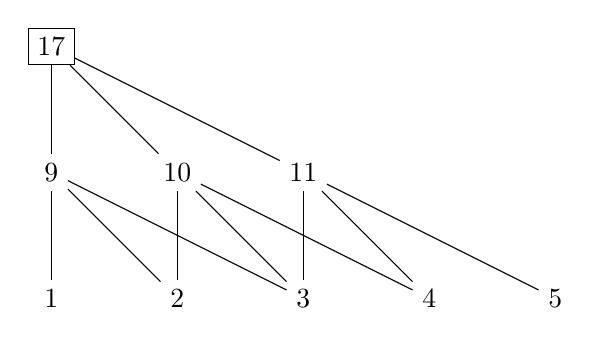
\begin{tikzpicture}
  \node[minimum size=0.3cm] (1) at (0.00,-3.20) {1};
  \node[minimum size=0.3cm] (2) at (1.60,-3.20) {2};
  \node[minimum size=0.3cm] (3) at (3.20,-3.20) {3};
  \node[minimum size=0.3cm] (4) at (4.80,-3.20) {4};
  \node[minimum size=0.3cm] (5) at (6.40,-3.20) {5};
  \node[minimum size=0.3cm] (9) at (0.00,-1.60) {9};
  \node[minimum size=0.3cm] (10) at (1.60,-1.60) {10};
  \node[minimum size=0.3cm] (11) at (3.20,-1.60) {11};
  \node[draw, rectangle, minimum size=0.3cm] (17) at (0.00,0.00) {17};
  % Draw the cover relations
  \draw (9) -- (3);
  \draw (17) -- (10);
  \draw (10) -- (4);
  \draw (11) -- (3);
  \draw (9) -- (2);
  \draw (17) -- (9);
  \draw (11) -- (5);
  \draw (10) -- (3);
  \draw (17) -- (11);
  \draw (9) -- (1);
  \draw (11) -- (4);
  \draw (10) -- (2);
\end{tikzpicture}
\end{minipage}%
\hfill\begin{minipage}{0.48\textwidth}
\subsubsection*{Void Poset}
\centering
\end{minipage}
\newpage\subsection{[6, 8, 10, 13]}
\noindent\begin{minipage}{0.6\textwidth}
\subsubsection*{Invariants}
\centering
\begin{tabular}{|c|c|c|c|c|c|c|}
\toprule
g & F & m & ewt & t & \(|M|\) & \(|\lambda|\) \\
\midrule
10 & 17 & 6 & 14 & 2 & 2 & 29 \\
\bottomrule
\end{tabular}
\end{minipage}%
\begin{minipage}{0.4\textwidth}
\subsubsection*{Partition}
\centering
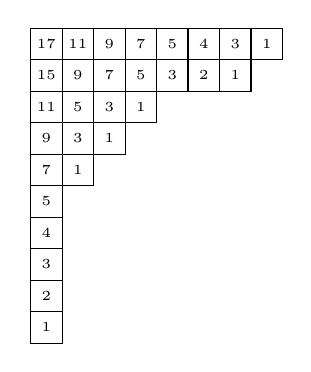
\begin{tikzpicture}
  \draw (0.00, 0.00) rectangle (0.40, -0.40);
  \node[font=\tiny] at (0.20, -0.20) {17};
  \draw (0.40, 0.00) rectangle (0.80, -0.40);
  \node[font=\tiny] at (0.60, -0.20) {11};
  \draw (0.80, 0.00) rectangle (1.20, -0.40);
  \node[font=\tiny] at (1.00, -0.20) {9};
  \draw (1.20, 0.00) rectangle (1.60, -0.40);
  \node[font=\tiny] at (1.40, -0.20) {7};
  \draw (1.60, 0.00) rectangle (2.00, -0.40);
  \node[font=\tiny] at (1.80, -0.20) {5};
  \draw (2.00, 0.00) rectangle (2.40, -0.40);
  \node[font=\tiny] at (2.20, -0.20) {4};
  \draw (2.40, 0.00) rectangle (2.80, -0.40);
  \node[font=\tiny] at (2.60, -0.20) {3};
  \draw (2.80, 0.00) rectangle (3.20, -0.40);
  \node[font=\tiny] at (3.00, -0.20) {1};
  \draw (0.00, -0.40) rectangle (0.40, -0.80);
  \node[font=\tiny] at (0.20, -0.60) {15};
  \draw (0.40, -0.40) rectangle (0.80, -0.80);
  \node[font=\tiny] at (0.60, -0.60) {9};
  \draw (0.80, -0.40) rectangle (1.20, -0.80);
  \node[font=\tiny] at (1.00, -0.60) {7};
  \draw (1.20, -0.40) rectangle (1.60, -0.80);
  \node[font=\tiny] at (1.40, -0.60) {5};
  \draw (1.60, -0.40) rectangle (2.00, -0.80);
  \node[font=\tiny] at (1.80, -0.60) {3};
  \draw (2.00, -0.40) rectangle (2.40, -0.80);
  \node[font=\tiny] at (2.20, -0.60) {2};
  \draw (2.40, -0.40) rectangle (2.80, -0.80);
  \node[font=\tiny] at (2.60, -0.60) {1};
  \draw (0.00, -0.80) rectangle (0.40, -1.20);
  \node[font=\tiny] at (0.20, -1.00) {11};
  \draw (0.40, -0.80) rectangle (0.80, -1.20);
  \node[font=\tiny] at (0.60, -1.00) {5};
  \draw (0.80, -0.80) rectangle (1.20, -1.20);
  \node[font=\tiny] at (1.00, -1.00) {3};
  \draw (1.20, -0.80) rectangle (1.60, -1.20);
  \node[font=\tiny] at (1.40, -1.00) {1};
  \draw (0.00, -1.20) rectangle (0.40, -1.60);
  \node[font=\tiny] at (0.20, -1.40) {9};
  \draw (0.40, -1.20) rectangle (0.80, -1.60);
  \node[font=\tiny] at (0.60, -1.40) {3};
  \draw (0.80, -1.20) rectangle (1.20, -1.60);
  \node[font=\tiny] at (1.00, -1.40) {1};
  \draw (0.00, -1.60) rectangle (0.40, -2.00);
  \node[font=\tiny] at (0.20, -1.80) {7};
  \draw (0.40, -1.60) rectangle (0.80, -2.00);
  \node[font=\tiny] at (0.60, -1.80) {1};
  \draw (0.00, -2.00) rectangle (0.40, -2.40);
  \node[font=\tiny] at (0.20, -2.20) {5};
  \draw (0.00, -2.40) rectangle (0.40, -2.80);
  \node[font=\tiny] at (0.20, -2.60) {4};
  \draw (0.00, -2.80) rectangle (0.40, -3.20);
  \node[font=\tiny] at (0.20, -3.00) {3};
  \draw (0.00, -3.20) rectangle (0.40, -3.60);
  \node[font=\tiny] at (0.20, -3.40) {2};
  \draw (0.00, -3.60) rectangle (0.40, -4.00);
  \node[font=\tiny] at (0.20, -3.80) {1};
\end{tikzpicture}
\end{minipage}
\vspace{1cm}
\noindent \newline\begin{minipage}{0.48\textwidth}
\subsubsection*{Gap Poset}
\centering
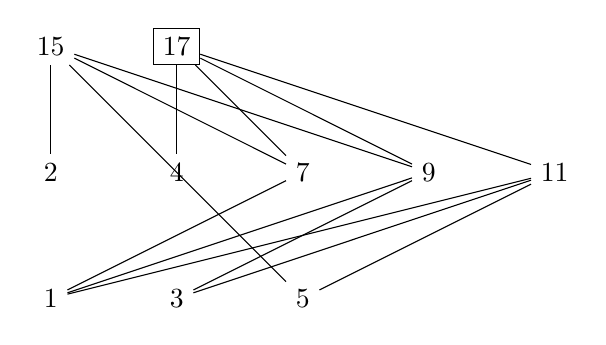
\begin{tikzpicture}
  \node[minimum size=0.3cm] (1) at (0.00,-3.20) {1};
  \node[minimum size=0.3cm] (3) at (1.60,-3.20) {3};
  \node[minimum size=0.3cm] (5) at (3.20,-3.20) {5};
  \node[minimum size=0.3cm] (2) at (0.00,-1.60) {2};
  \node[minimum size=0.3cm] (4) at (1.60,-1.60) {4};
  \node[minimum size=0.3cm] (7) at (3.20,-1.60) {7};
  \node[minimum size=0.3cm] (9) at (4.80,-1.60) {9};
  \node[minimum size=0.3cm] (11) at (6.40,-1.60) {11};
  \node[minimum size=0.3cm] (15) at (0.00,0.00) {15};
  \node[draw, rectangle, minimum size=0.3cm] (17) at (1.60,0.00) {17};
  % Draw the cover relations
  \draw (11) -- (1);
  \draw (15) -- (5);
  \draw (17) -- (7);
  \draw (7) -- (1);
  \draw (9) -- (3);
  \draw (11) -- (3);
  \draw (15) -- (7);
  \draw (17) -- (9);
  \draw (11) -- (5);
  \draw (15) -- (9);
  \draw (17) -- (11);
  \draw (9) -- (1);
  \draw (15) -- (2);
  \draw (17) -- (4);
\end{tikzpicture}
\end{minipage}%
\hfill\begin{minipage}{0.48\textwidth}
\subsubsection*{Void Poset}
\centering
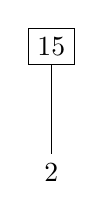
\begin{tikzpicture}
  \node[minimum size=0.3cm] (2) at (0.00,-1.60) {2};
  \node[draw, rectangle, minimum size=0.3cm] (15) at (0.00,0.00) {15};
  % Draw the cover relations
  \draw (15) -- (2);
\end{tikzpicture}
\end{minipage}
\newpage\subsection{[8, 10, 11, 12, 13]}
\noindent\begin{minipage}{0.6\textwidth}
\subsubsection*{Invariants}
\centering
\begin{tabular}{|c|c|c|c|c|c|c|}
\toprule
g & F & m & ewt & t & \(|M|\) & \(|\lambda|\) \\
\midrule
11 & 17 & 8 & 16 & 3 & 4 & 28 \\
\bottomrule
\end{tabular}
\end{minipage}%
\begin{minipage}{0.4\textwidth}
\subsubsection*{Partition}
\centering
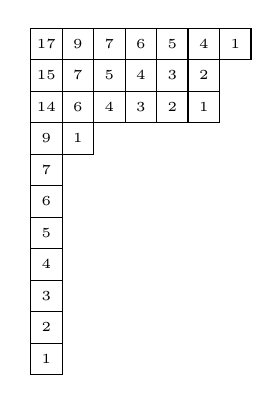
\begin{tikzpicture}
  \draw (0.00, 0.00) rectangle (0.40, -0.40);
  \node[font=\tiny] at (0.20, -0.20) {17};
  \draw (0.40, 0.00) rectangle (0.80, -0.40);
  \node[font=\tiny] at (0.60, -0.20) {9};
  \draw (0.80, 0.00) rectangle (1.20, -0.40);
  \node[font=\tiny] at (1.00, -0.20) {7};
  \draw (1.20, 0.00) rectangle (1.60, -0.40);
  \node[font=\tiny] at (1.40, -0.20) {6};
  \draw (1.60, 0.00) rectangle (2.00, -0.40);
  \node[font=\tiny] at (1.80, -0.20) {5};
  \draw (2.00, 0.00) rectangle (2.40, -0.40);
  \node[font=\tiny] at (2.20, -0.20) {4};
  \draw (2.40, 0.00) rectangle (2.80, -0.40);
  \node[font=\tiny] at (2.60, -0.20) {1};
  \draw (0.00, -0.40) rectangle (0.40, -0.80);
  \node[font=\tiny] at (0.20, -0.60) {15};
  \draw (0.40, -0.40) rectangle (0.80, -0.80);
  \node[font=\tiny] at (0.60, -0.60) {7};
  \draw (0.80, -0.40) rectangle (1.20, -0.80);
  \node[font=\tiny] at (1.00, -0.60) {5};
  \draw (1.20, -0.40) rectangle (1.60, -0.80);
  \node[font=\tiny] at (1.40, -0.60) {4};
  \draw (1.60, -0.40) rectangle (2.00, -0.80);
  \node[font=\tiny] at (1.80, -0.60) {3};
  \draw (2.00, -0.40) rectangle (2.40, -0.80);
  \node[font=\tiny] at (2.20, -0.60) {2};
  \draw (0.00, -0.80) rectangle (0.40, -1.20);
  \node[font=\tiny] at (0.20, -1.00) {14};
  \draw (0.40, -0.80) rectangle (0.80, -1.20);
  \node[font=\tiny] at (0.60, -1.00) {6};
  \draw (0.80, -0.80) rectangle (1.20, -1.20);
  \node[font=\tiny] at (1.00, -1.00) {4};
  \draw (1.20, -0.80) rectangle (1.60, -1.20);
  \node[font=\tiny] at (1.40, -1.00) {3};
  \draw (1.60, -0.80) rectangle (2.00, -1.20);
  \node[font=\tiny] at (1.80, -1.00) {2};
  \draw (2.00, -0.80) rectangle (2.40, -1.20);
  \node[font=\tiny] at (2.20, -1.00) {1};
  \draw (0.00, -1.20) rectangle (0.40, -1.60);
  \node[font=\tiny] at (0.20, -1.40) {9};
  \draw (0.40, -1.20) rectangle (0.80, -1.60);
  \node[font=\tiny] at (0.60, -1.40) {1};
  \draw (0.00, -1.60) rectangle (0.40, -2.00);
  \node[font=\tiny] at (0.20, -1.80) {7};
  \draw (0.00, -2.00) rectangle (0.40, -2.40);
  \node[font=\tiny] at (0.20, -2.20) {6};
  \draw (0.00, -2.40) rectangle (0.40, -2.80);
  \node[font=\tiny] at (0.20, -2.60) {5};
  \draw (0.00, -2.80) rectangle (0.40, -3.20);
  \node[font=\tiny] at (0.20, -3.00) {4};
  \draw (0.00, -3.20) rectangle (0.40, -3.60);
  \node[font=\tiny] at (0.20, -3.40) {3};
  \draw (0.00, -3.60) rectangle (0.40, -4.00);
  \node[font=\tiny] at (0.20, -3.80) {2};
  \draw (0.00, -4.00) rectangle (0.40, -4.40);
  \node[font=\tiny] at (0.20, -4.20) {1};
\end{tikzpicture}
\end{minipage}
\vspace{1cm}
\noindent \newline\begin{minipage}{0.48\textwidth}
\subsubsection*{Gap Poset}
\centering
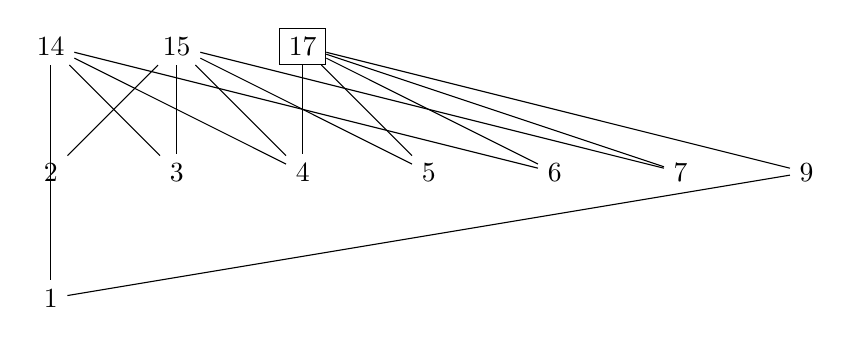
\begin{tikzpicture}
  \node[minimum size=0.3cm] (1) at (0.00,-3.20) {1};
  \node[minimum size=0.3cm] (2) at (0.00,-1.60) {2};
  \node[minimum size=0.3cm] (3) at (1.60,-1.60) {3};
  \node[minimum size=0.3cm] (4) at (3.20,-1.60) {4};
  \node[minimum size=0.3cm] (5) at (4.80,-1.60) {5};
  \node[minimum size=0.3cm] (6) at (6.40,-1.60) {6};
  \node[minimum size=0.3cm] (7) at (8.00,-1.60) {7};
  \node[minimum size=0.3cm] (9) at (9.60,-1.60) {9};
  \node[minimum size=0.3cm] (14) at (0.00,0.00) {14};
  \node[minimum size=0.3cm] (15) at (1.60,0.00) {15};
  \node[draw, rectangle, minimum size=0.3cm] (17) at (3.20,0.00) {17};
  % Draw the cover relations
  \draw (15) -- (5);
  \draw (17) -- (7);
  \draw (14) -- (4);
  \draw (14) -- (1);
  \draw (15) -- (4);
  \draw (15) -- (7);
  \draw (17) -- (9);
  \draw (14) -- (6);
  \draw (17) -- (6);
  \draw (14) -- (3);
  \draw (15) -- (3);
  \draw (17) -- (5);
  \draw (14) -- (2);
  \draw (9) -- (1);
  \draw (15) -- (2);
  \draw (17) -- (4);
\end{tikzpicture}
\end{minipage}%
\hfill\begin{minipage}{0.48\textwidth}
\subsubsection*{Void Poset}
\centering
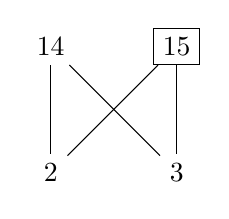
\begin{tikzpicture}
  \node[minimum size=0.3cm] (2) at (0.00,-1.60) {2};
  \node[minimum size=0.3cm] (3) at (1.60,-1.60) {3};
  \node[minimum size=0.3cm] (14) at (0.00,0.00) {14};
  \node[draw, rectangle, minimum size=0.3cm] (15) at (1.60,0.00) {15};
  % Draw the cover relations
  \draw (14) -- (2);
  \draw (14) -- (3);
  \draw (15) -- (2);
  \draw (15) -- (3);
\end{tikzpicture}
\end{minipage}
\newpage\subsection{[7, 9, 11, 13, 15]}
\noindent\begin{minipage}{0.6\textwidth}
\subsubsection*{Invariants}
\centering
\begin{tabular}{|c|c|c|c|c|c|c|}
\toprule
g & F & m & ewt & t & \(|M|\) & \(|\lambda|\) \\
\midrule
11 & 19 & 7 & 16 & 2 & 2 & 32 \\
\bottomrule
\end{tabular}
\end{minipage}%
\begin{minipage}{0.4\textwidth}
\subsubsection*{Partition}
\centering
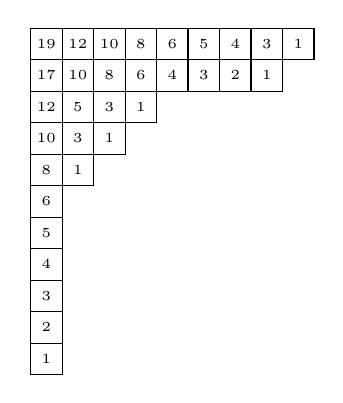
\begin{tikzpicture}
  \draw (0.00, 0.00) rectangle (0.40, -0.40);
  \node[font=\tiny] at (0.20, -0.20) {19};
  \draw (0.40, 0.00) rectangle (0.80, -0.40);
  \node[font=\tiny] at (0.60, -0.20) {12};
  \draw (0.80, 0.00) rectangle (1.20, -0.40);
  \node[font=\tiny] at (1.00, -0.20) {10};
  \draw (1.20, 0.00) rectangle (1.60, -0.40);
  \node[font=\tiny] at (1.40, -0.20) {8};
  \draw (1.60, 0.00) rectangle (2.00, -0.40);
  \node[font=\tiny] at (1.80, -0.20) {6};
  \draw (2.00, 0.00) rectangle (2.40, -0.40);
  \node[font=\tiny] at (2.20, -0.20) {5};
  \draw (2.40, 0.00) rectangle (2.80, -0.40);
  \node[font=\tiny] at (2.60, -0.20) {4};
  \draw (2.80, 0.00) rectangle (3.20, -0.40);
  \node[font=\tiny] at (3.00, -0.20) {3};
  \draw (3.20, 0.00) rectangle (3.60, -0.40);
  \node[font=\tiny] at (3.40, -0.20) {1};
  \draw (0.00, -0.40) rectangle (0.40, -0.80);
  \node[font=\tiny] at (0.20, -0.60) {17};
  \draw (0.40, -0.40) rectangle (0.80, -0.80);
  \node[font=\tiny] at (0.60, -0.60) {10};
  \draw (0.80, -0.40) rectangle (1.20, -0.80);
  \node[font=\tiny] at (1.00, -0.60) {8};
  \draw (1.20, -0.40) rectangle (1.60, -0.80);
  \node[font=\tiny] at (1.40, -0.60) {6};
  \draw (1.60, -0.40) rectangle (2.00, -0.80);
  \node[font=\tiny] at (1.80, -0.60) {4};
  \draw (2.00, -0.40) rectangle (2.40, -0.80);
  \node[font=\tiny] at (2.20, -0.60) {3};
  \draw (2.40, -0.40) rectangle (2.80, -0.80);
  \node[font=\tiny] at (2.60, -0.60) {2};
  \draw (2.80, -0.40) rectangle (3.20, -0.80);
  \node[font=\tiny] at (3.00, -0.60) {1};
  \draw (0.00, -0.80) rectangle (0.40, -1.20);
  \node[font=\tiny] at (0.20, -1.00) {12};
  \draw (0.40, -0.80) rectangle (0.80, -1.20);
  \node[font=\tiny] at (0.60, -1.00) {5};
  \draw (0.80, -0.80) rectangle (1.20, -1.20);
  \node[font=\tiny] at (1.00, -1.00) {3};
  \draw (1.20, -0.80) rectangle (1.60, -1.20);
  \node[font=\tiny] at (1.40, -1.00) {1};
  \draw (0.00, -1.20) rectangle (0.40, -1.60);
  \node[font=\tiny] at (0.20, -1.40) {10};
  \draw (0.40, -1.20) rectangle (0.80, -1.60);
  \node[font=\tiny] at (0.60, -1.40) {3};
  \draw (0.80, -1.20) rectangle (1.20, -1.60);
  \node[font=\tiny] at (1.00, -1.40) {1};
  \draw (0.00, -1.60) rectangle (0.40, -2.00);
  \node[font=\tiny] at (0.20, -1.80) {8};
  \draw (0.40, -1.60) rectangle (0.80, -2.00);
  \node[font=\tiny] at (0.60, -1.80) {1};
  \draw (0.00, -2.00) rectangle (0.40, -2.40);
  \node[font=\tiny] at (0.20, -2.20) {6};
  \draw (0.00, -2.40) rectangle (0.40, -2.80);
  \node[font=\tiny] at (0.20, -2.60) {5};
  \draw (0.00, -2.80) rectangle (0.40, -3.20);
  \node[font=\tiny] at (0.20, -3.00) {4};
  \draw (0.00, -3.20) rectangle (0.40, -3.60);
  \node[font=\tiny] at (0.20, -3.40) {3};
  \draw (0.00, -3.60) rectangle (0.40, -4.00);
  \node[font=\tiny] at (0.20, -3.80) {2};
  \draw (0.00, -4.00) rectangle (0.40, -4.40);
  \node[font=\tiny] at (0.20, -4.20) {1};
\end{tikzpicture}
\end{minipage}
\vspace{1cm}
\noindent \newline\begin{minipage}{0.48\textwidth}
\subsubsection*{Gap Poset}
\centering
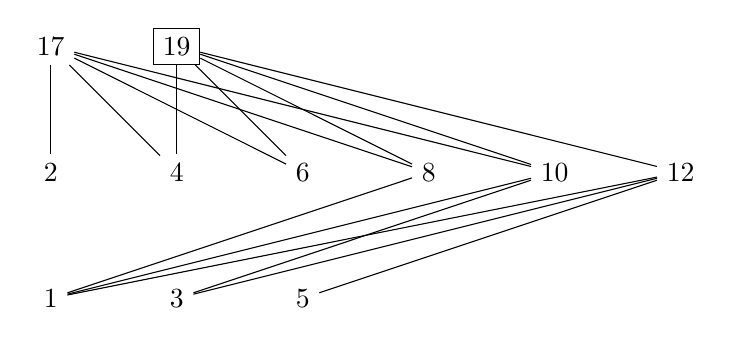
\begin{tikzpicture}
  \node[minimum size=0.3cm] (1) at (0.00,-3.20) {1};
  \node[minimum size=0.3cm] (3) at (1.60,-3.20) {3};
  \node[minimum size=0.3cm] (5) at (3.20,-3.20) {5};
  \node[minimum size=0.3cm] (2) at (0.00,-1.60) {2};
  \node[minimum size=0.3cm] (4) at (1.60,-1.60) {4};
  \node[minimum size=0.3cm] (6) at (3.20,-1.60) {6};
  \node[minimum size=0.3cm] (8) at (4.80,-1.60) {8};
  \node[minimum size=0.3cm] (10) at (6.40,-1.60) {10};
  \node[minimum size=0.3cm] (12) at (8.00,-1.60) {12};
  \node[minimum size=0.3cm] (17) at (0.00,0.00) {17};
  \node[draw, rectangle, minimum size=0.3cm] (19) at (1.60,0.00) {19};
  % Draw the cover relations
  \draw (19) -- (8);
  \draw (12) -- (1);
  \draw (19) -- (4);
  \draw (8) -- (1);
  \draw (17) -- (10);
  \draw (10) -- (1);
  \draw (19) -- (10);
  \draw (12) -- (3);
  \draw (19) -- (6);
  \draw (17) -- (6);
  \draw (17) -- (2);
  \draw (19) -- (12);
  \draw (12) -- (5);
  \draw (17) -- (8);
  \draw (10) -- (3);
  \draw (17) -- (4);
\end{tikzpicture}
\end{minipage}%
\hfill\begin{minipage}{0.48\textwidth}
\subsubsection*{Void Poset}
\centering
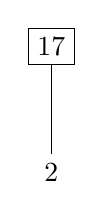
\begin{tikzpicture}
  \node[draw, rectangle, minimum size=0.3cm] (17) at (0.00,0.00) {17};
  \node[minimum size=0.3cm] (2) at (0.00,-1.60) {2};
  % Draw the cover relations
  \draw (17) -- (2);
\end{tikzpicture}
\end{minipage}
\newpage\subsection{[7, 8, 9, 19]}
\noindent\begin{minipage}{0.6\textwidth}
\subsubsection*{Invariants}
\centering
\begin{tabular}{|c|c|c|c|c|c|c|}
\toprule
g & F & m & ewt & t & \(|M|\) & \(|\lambda|\) \\
\midrule
11 & 20 & 7 & 16 & 2 & 1 & 32 \\
\bottomrule
\end{tabular}
\end{minipage}%
\begin{minipage}{0.4\textwidth}
\subsubsection*{Partition}
\centering
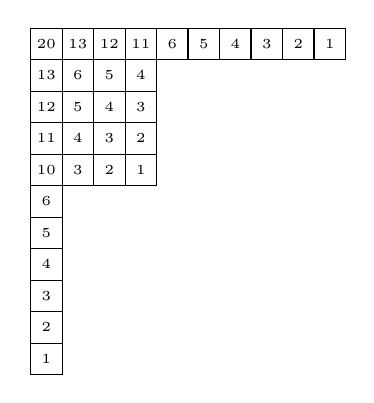
\begin{tikzpicture}
  \draw (0.00, 0.00) rectangle (0.40, -0.40);
  \node[font=\tiny] at (0.20, -0.20) {20};
  \draw (0.40, 0.00) rectangle (0.80, -0.40);
  \node[font=\tiny] at (0.60, -0.20) {13};
  \draw (0.80, 0.00) rectangle (1.20, -0.40);
  \node[font=\tiny] at (1.00, -0.20) {12};
  \draw (1.20, 0.00) rectangle (1.60, -0.40);
  \node[font=\tiny] at (1.40, -0.20) {11};
  \draw (1.60, 0.00) rectangle (2.00, -0.40);
  \node[font=\tiny] at (1.80, -0.20) {6};
  \draw (2.00, 0.00) rectangle (2.40, -0.40);
  \node[font=\tiny] at (2.20, -0.20) {5};
  \draw (2.40, 0.00) rectangle (2.80, -0.40);
  \node[font=\tiny] at (2.60, -0.20) {4};
  \draw (2.80, 0.00) rectangle (3.20, -0.40);
  \node[font=\tiny] at (3.00, -0.20) {3};
  \draw (3.20, 0.00) rectangle (3.60, -0.40);
  \node[font=\tiny] at (3.40, -0.20) {2};
  \draw (3.60, 0.00) rectangle (4.00, -0.40);
  \node[font=\tiny] at (3.80, -0.20) {1};
  \draw (0.00, -0.40) rectangle (0.40, -0.80);
  \node[font=\tiny] at (0.20, -0.60) {13};
  \draw (0.40, -0.40) rectangle (0.80, -0.80);
  \node[font=\tiny] at (0.60, -0.60) {6};
  \draw (0.80, -0.40) rectangle (1.20, -0.80);
  \node[font=\tiny] at (1.00, -0.60) {5};
  \draw (1.20, -0.40) rectangle (1.60, -0.80);
  \node[font=\tiny] at (1.40, -0.60) {4};
  \draw (0.00, -0.80) rectangle (0.40, -1.20);
  \node[font=\tiny] at (0.20, -1.00) {12};
  \draw (0.40, -0.80) rectangle (0.80, -1.20);
  \node[font=\tiny] at (0.60, -1.00) {5};
  \draw (0.80, -0.80) rectangle (1.20, -1.20);
  \node[font=\tiny] at (1.00, -1.00) {4};
  \draw (1.20, -0.80) rectangle (1.60, -1.20);
  \node[font=\tiny] at (1.40, -1.00) {3};
  \draw (0.00, -1.20) rectangle (0.40, -1.60);
  \node[font=\tiny] at (0.20, -1.40) {11};
  \draw (0.40, -1.20) rectangle (0.80, -1.60);
  \node[font=\tiny] at (0.60, -1.40) {4};
  \draw (0.80, -1.20) rectangle (1.20, -1.60);
  \node[font=\tiny] at (1.00, -1.40) {3};
  \draw (1.20, -1.20) rectangle (1.60, -1.60);
  \node[font=\tiny] at (1.40, -1.40) {2};
  \draw (0.00, -1.60) rectangle (0.40, -2.00);
  \node[font=\tiny] at (0.20, -1.80) {10};
  \draw (0.40, -1.60) rectangle (0.80, -2.00);
  \node[font=\tiny] at (0.60, -1.80) {3};
  \draw (0.80, -1.60) rectangle (1.20, -2.00);
  \node[font=\tiny] at (1.00, -1.80) {2};
  \draw (1.20, -1.60) rectangle (1.60, -2.00);
  \node[font=\tiny] at (1.40, -1.80) {1};
  \draw (0.00, -2.00) rectangle (0.40, -2.40);
  \node[font=\tiny] at (0.20, -2.20) {6};
  \draw (0.00, -2.40) rectangle (0.40, -2.80);
  \node[font=\tiny] at (0.20, -2.60) {5};
  \draw (0.00, -2.80) rectangle (0.40, -3.20);
  \node[font=\tiny] at (0.20, -3.00) {4};
  \draw (0.00, -3.20) rectangle (0.40, -3.60);
  \node[font=\tiny] at (0.20, -3.40) {3};
  \draw (0.00, -3.60) rectangle (0.40, -4.00);
  \node[font=\tiny] at (0.20, -3.80) {2};
  \draw (0.00, -4.00) rectangle (0.40, -4.40);
  \node[font=\tiny] at (0.20, -4.20) {1};
\end{tikzpicture}
\end{minipage}
\vspace{1cm}
\noindent \newline\begin{minipage}{0.48\textwidth}
\subsubsection*{Gap Poset}
\centering
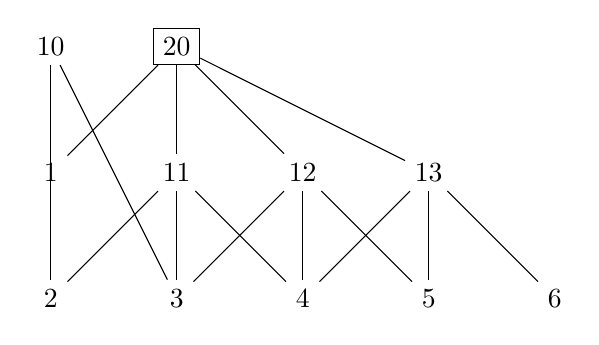
\begin{tikzpicture}
  \node[minimum size=0.3cm] (1) at (0.00,-1.60) {1};
  \node[minimum size=0.3cm] (11) at (1.60,-1.60) {11};
  \node[minimum size=0.3cm] (12) at (3.20,-1.60) {12};
  \node[minimum size=0.3cm] (13) at (4.80,-1.60) {13};
  \node[minimum size=0.3cm] (2) at (0.00,-3.20) {2};
  \node[minimum size=0.3cm] (3) at (1.60,-3.20) {3};
  \node[minimum size=0.3cm] (4) at (3.20,-3.20) {4};
  \node[minimum size=0.3cm] (5) at (4.80,-3.20) {5};
  \node[minimum size=0.3cm] (6) at (6.40,-3.20) {6};
  \node[minimum size=0.3cm] (10) at (0.00,0.00) {10};
  \node[draw, rectangle, minimum size=0.3cm] (20) at (1.60,0.00) {20};
  % Draw the cover relations
  \draw (12) -- (4);
  \draw (20) -- (11);
  \draw (13) -- (4);
  \draw (20) -- (1);
  \draw (11) -- (3);
  \draw (20) -- (13);
  \draw (10) -- (1);
  \draw (12) -- (3);
  \draw (11) -- (2);
  \draw (13) -- (6);
  \draw (10) -- (3);
  \draw (12) -- (5);
  \draw (20) -- (12);
  \draw (13) -- (5);
  \draw (11) -- (4);
  \draw (10) -- (2);
\end{tikzpicture}
\end{minipage}%
\hfill\begin{minipage}{0.48\textwidth}
\subsubsection*{Void Poset}
\centering
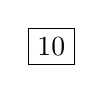
\begin{tikzpicture}
  \node[draw, rectangle, minimum size=0.3cm] (10) at (0.00,0.00) {10};
\end{tikzpicture}
\end{minipage}
\newpage\subsection{[8, 9, 10, 11]}
\noindent\begin{minipage}{0.6\textwidth}
\subsubsection*{Invariants}
\centering
\begin{tabular}{|c|c|c|c|c|c|c|}
\toprule
g & F & m & ewt & t & \(|M|\) & \(|\lambda|\) \\
\midrule
12 & 23 & 8 & 20 & 1 & 0 & 39 \\
\bottomrule
\end{tabular}
\end{minipage}%
\begin{minipage}{0.4\textwidth}
\subsubsection*{Partition}
\centering
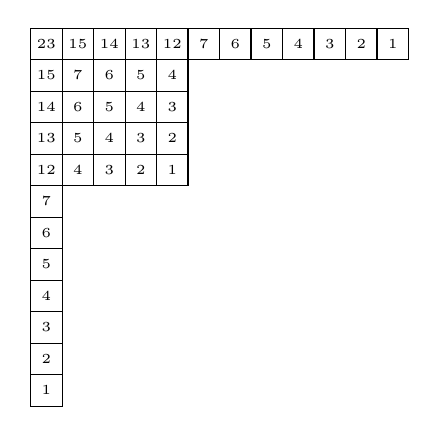
\begin{tikzpicture}
  \draw (0.00, 0.00) rectangle (0.40, -0.40);
  \node[font=\tiny] at (0.20, -0.20) {23};
  \draw (0.40, 0.00) rectangle (0.80, -0.40);
  \node[font=\tiny] at (0.60, -0.20) {15};
  \draw (0.80, 0.00) rectangle (1.20, -0.40);
  \node[font=\tiny] at (1.00, -0.20) {14};
  \draw (1.20, 0.00) rectangle (1.60, -0.40);
  \node[font=\tiny] at (1.40, -0.20) {13};
  \draw (1.60, 0.00) rectangle (2.00, -0.40);
  \node[font=\tiny] at (1.80, -0.20) {12};
  \draw (2.00, 0.00) rectangle (2.40, -0.40);
  \node[font=\tiny] at (2.20, -0.20) {7};
  \draw (2.40, 0.00) rectangle (2.80, -0.40);
  \node[font=\tiny] at (2.60, -0.20) {6};
  \draw (2.80, 0.00) rectangle (3.20, -0.40);
  \node[font=\tiny] at (3.00, -0.20) {5};
  \draw (3.20, 0.00) rectangle (3.60, -0.40);
  \node[font=\tiny] at (3.40, -0.20) {4};
  \draw (3.60, 0.00) rectangle (4.00, -0.40);
  \node[font=\tiny] at (3.80, -0.20) {3};
  \draw (4.00, 0.00) rectangle (4.40, -0.40);
  \node[font=\tiny] at (4.20, -0.20) {2};
  \draw (4.40, 0.00) rectangle (4.80, -0.40);
  \node[font=\tiny] at (4.60, -0.20) {1};
  \draw (0.00, -0.40) rectangle (0.40, -0.80);
  \node[font=\tiny] at (0.20, -0.60) {15};
  \draw (0.40, -0.40) rectangle (0.80, -0.80);
  \node[font=\tiny] at (0.60, -0.60) {7};
  \draw (0.80, -0.40) rectangle (1.20, -0.80);
  \node[font=\tiny] at (1.00, -0.60) {6};
  \draw (1.20, -0.40) rectangle (1.60, -0.80);
  \node[font=\tiny] at (1.40, -0.60) {5};
  \draw (1.60, -0.40) rectangle (2.00, -0.80);
  \node[font=\tiny] at (1.80, -0.60) {4};
  \draw (0.00, -0.80) rectangle (0.40, -1.20);
  \node[font=\tiny] at (0.20, -1.00) {14};
  \draw (0.40, -0.80) rectangle (0.80, -1.20);
  \node[font=\tiny] at (0.60, -1.00) {6};
  \draw (0.80, -0.80) rectangle (1.20, -1.20);
  \node[font=\tiny] at (1.00, -1.00) {5};
  \draw (1.20, -0.80) rectangle (1.60, -1.20);
  \node[font=\tiny] at (1.40, -1.00) {4};
  \draw (1.60, -0.80) rectangle (2.00, -1.20);
  \node[font=\tiny] at (1.80, -1.00) {3};
  \draw (0.00, -1.20) rectangle (0.40, -1.60);
  \node[font=\tiny] at (0.20, -1.40) {13};
  \draw (0.40, -1.20) rectangle (0.80, -1.60);
  \node[font=\tiny] at (0.60, -1.40) {5};
  \draw (0.80, -1.20) rectangle (1.20, -1.60);
  \node[font=\tiny] at (1.00, -1.40) {4};
  \draw (1.20, -1.20) rectangle (1.60, -1.60);
  \node[font=\tiny] at (1.40, -1.40) {3};
  \draw (1.60, -1.20) rectangle (2.00, -1.60);
  \node[font=\tiny] at (1.80, -1.40) {2};
  \draw (0.00, -1.60) rectangle (0.40, -2.00);
  \node[font=\tiny] at (0.20, -1.80) {12};
  \draw (0.40, -1.60) rectangle (0.80, -2.00);
  \node[font=\tiny] at (0.60, -1.80) {4};
  \draw (0.80, -1.60) rectangle (1.20, -2.00);
  \node[font=\tiny] at (1.00, -1.80) {3};
  \draw (1.20, -1.60) rectangle (1.60, -2.00);
  \node[font=\tiny] at (1.40, -1.80) {2};
  \draw (1.60, -1.60) rectangle (2.00, -2.00);
  \node[font=\tiny] at (1.80, -1.80) {1};
  \draw (0.00, -2.00) rectangle (0.40, -2.40);
  \node[font=\tiny] at (0.20, -2.20) {7};
  \draw (0.00, -2.40) rectangle (0.40, -2.80);
  \node[font=\tiny] at (0.20, -2.60) {6};
  \draw (0.00, -2.80) rectangle (0.40, -3.20);
  \node[font=\tiny] at (0.20, -3.00) {5};
  \draw (0.00, -3.20) rectangle (0.40, -3.60);
  \node[font=\tiny] at (0.20, -3.40) {4};
  \draw (0.00, -3.60) rectangle (0.40, -4.00);
  \node[font=\tiny] at (0.20, -3.80) {3};
  \draw (0.00, -4.00) rectangle (0.40, -4.40);
  \node[font=\tiny] at (0.20, -4.20) {2};
  \draw (0.00, -4.40) rectangle (0.40, -4.80);
  \node[font=\tiny] at (0.20, -4.60) {1};
\end{tikzpicture}
\end{minipage}
\vspace{1cm}
\noindent \newline\begin{minipage}{0.48\textwidth}
\subsubsection*{Gap Poset}
\centering
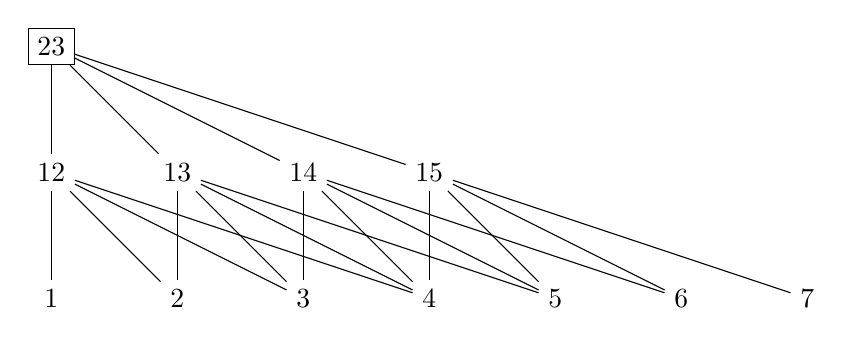
\begin{tikzpicture}
  \node[minimum size=0.3cm] (1) at (0.00,-3.20) {1};
  \node[minimum size=0.3cm] (2) at (1.60,-3.20) {2};
  \node[minimum size=0.3cm] (3) at (3.20,-3.20) {3};
  \node[minimum size=0.3cm] (4) at (4.80,-3.20) {4};
  \node[minimum size=0.3cm] (5) at (6.40,-3.20) {5};
  \node[minimum size=0.3cm] (6) at (8.00,-3.20) {6};
  \node[minimum size=0.3cm] (7) at (9.60,-3.20) {7};
  \node[minimum size=0.3cm] (12) at (0.00,-1.60) {12};
  \node[minimum size=0.3cm] (13) at (1.60,-1.60) {13};
  \node[minimum size=0.3cm] (14) at (3.20,-1.60) {14};
  \node[minimum size=0.3cm] (15) at (4.80,-1.60) {15};
  \node[draw, rectangle, minimum size=0.3cm] (23) at (0.00,0.00) {23};
  % Draw the cover relations
  \draw (12) -- (4);
  \draw (12) -- (1);
  \draw (14) -- (4);
  \draw (23) -- (13);
  \draw (13) -- (2);
  \draw (13) -- (5);
  \draw (15) -- (5);
  \draw (12) -- (3);
  \draw (14) -- (6);
  \draw (14) -- (3);
  \draw (23) -- (12);
  \draw (23) -- (15);
  \draw (13) -- (4);
  \draw (15) -- (4);
  \draw (15) -- (7);
  \draw (12) -- (2);
  \draw (23) -- (14);
  \draw (14) -- (5);
  \draw (13) -- (3);
  \draw (15) -- (6);
\end{tikzpicture}
\end{minipage}%
\hfill\begin{minipage}{0.48\textwidth}
\subsubsection*{Void Poset}
\centering
\end{minipage}
\newpage\subsection{[10, 12, 13, 14, 15, 16, 17]}
\noindent\begin{minipage}{0.6\textwidth}
\subsubsection*{Invariants}
\centering
\begin{tabular}{|c|c|c|c|c|c|c|}
\toprule
g & F & m & ewt & t & \(|M|\) & \(|\lambda|\) \\
\midrule
13 & 21 & 10 & 22 & 3 & 4 & 36 \\
\bottomrule
\end{tabular}
\end{minipage}%
\begin{minipage}{0.4\textwidth}
\subsubsection*{Partition}
\centering
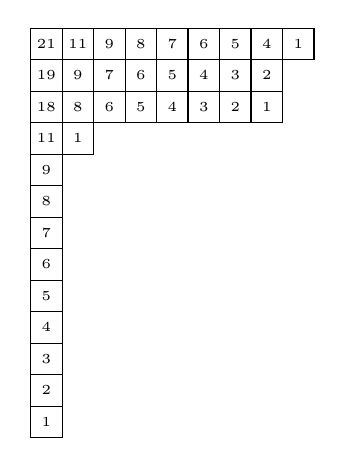
\begin{tikzpicture}
  \draw (0.00, 0.00) rectangle (0.40, -0.40);
  \node[font=\tiny] at (0.20, -0.20) {21};
  \draw (0.40, 0.00) rectangle (0.80, -0.40);
  \node[font=\tiny] at (0.60, -0.20) {11};
  \draw (0.80, 0.00) rectangle (1.20, -0.40);
  \node[font=\tiny] at (1.00, -0.20) {9};
  \draw (1.20, 0.00) rectangle (1.60, -0.40);
  \node[font=\tiny] at (1.40, -0.20) {8};
  \draw (1.60, 0.00) rectangle (2.00, -0.40);
  \node[font=\tiny] at (1.80, -0.20) {7};
  \draw (2.00, 0.00) rectangle (2.40, -0.40);
  \node[font=\tiny] at (2.20, -0.20) {6};
  \draw (2.40, 0.00) rectangle (2.80, -0.40);
  \node[font=\tiny] at (2.60, -0.20) {5};
  \draw (2.80, 0.00) rectangle (3.20, -0.40);
  \node[font=\tiny] at (3.00, -0.20) {4};
  \draw (3.20, 0.00) rectangle (3.60, -0.40);
  \node[font=\tiny] at (3.40, -0.20) {1};
  \draw (0.00, -0.40) rectangle (0.40, -0.80);
  \node[font=\tiny] at (0.20, -0.60) {19};
  \draw (0.40, -0.40) rectangle (0.80, -0.80);
  \node[font=\tiny] at (0.60, -0.60) {9};
  \draw (0.80, -0.40) rectangle (1.20, -0.80);
  \node[font=\tiny] at (1.00, -0.60) {7};
  \draw (1.20, -0.40) rectangle (1.60, -0.80);
  \node[font=\tiny] at (1.40, -0.60) {6};
  \draw (1.60, -0.40) rectangle (2.00, -0.80);
  \node[font=\tiny] at (1.80, -0.60) {5};
  \draw (2.00, -0.40) rectangle (2.40, -0.80);
  \node[font=\tiny] at (2.20, -0.60) {4};
  \draw (2.40, -0.40) rectangle (2.80, -0.80);
  \node[font=\tiny] at (2.60, -0.60) {3};
  \draw (2.80, -0.40) rectangle (3.20, -0.80);
  \node[font=\tiny] at (3.00, -0.60) {2};
  \draw (0.00, -0.80) rectangle (0.40, -1.20);
  \node[font=\tiny] at (0.20, -1.00) {18};
  \draw (0.40, -0.80) rectangle (0.80, -1.20);
  \node[font=\tiny] at (0.60, -1.00) {8};
  \draw (0.80, -0.80) rectangle (1.20, -1.20);
  \node[font=\tiny] at (1.00, -1.00) {6};
  \draw (1.20, -0.80) rectangle (1.60, -1.20);
  \node[font=\tiny] at (1.40, -1.00) {5};
  \draw (1.60, -0.80) rectangle (2.00, -1.20);
  \node[font=\tiny] at (1.80, -1.00) {4};
  \draw (2.00, -0.80) rectangle (2.40, -1.20);
  \node[font=\tiny] at (2.20, -1.00) {3};
  \draw (2.40, -0.80) rectangle (2.80, -1.20);
  \node[font=\tiny] at (2.60, -1.00) {2};
  \draw (2.80, -0.80) rectangle (3.20, -1.20);
  \node[font=\tiny] at (3.00, -1.00) {1};
  \draw (0.00, -1.20) rectangle (0.40, -1.60);
  \node[font=\tiny] at (0.20, -1.40) {11};
  \draw (0.40, -1.20) rectangle (0.80, -1.60);
  \node[font=\tiny] at (0.60, -1.40) {1};
  \draw (0.00, -1.60) rectangle (0.40, -2.00);
  \node[font=\tiny] at (0.20, -1.80) {9};
  \draw (0.00, -2.00) rectangle (0.40, -2.40);
  \node[font=\tiny] at (0.20, -2.20) {8};
  \draw (0.00, -2.40) rectangle (0.40, -2.80);
  \node[font=\tiny] at (0.20, -2.60) {7};
  \draw (0.00, -2.80) rectangle (0.40, -3.20);
  \node[font=\tiny] at (0.20, -3.00) {6};
  \draw (0.00, -3.20) rectangle (0.40, -3.60);
  \node[font=\tiny] at (0.20, -3.40) {5};
  \draw (0.00, -3.60) rectangle (0.40, -4.00);
  \node[font=\tiny] at (0.20, -3.80) {4};
  \draw (0.00, -4.00) rectangle (0.40, -4.40);
  \node[font=\tiny] at (0.20, -4.20) {3};
  \draw (0.00, -4.40) rectangle (0.40, -4.80);
  \node[font=\tiny] at (0.20, -4.60) {2};
  \draw (0.00, -4.80) rectangle (0.40, -5.20);
  \node[font=\tiny] at (0.20, -5.00) {1};
\end{tikzpicture}
\end{minipage}
\vspace{1cm}
\noindent \newline\begin{minipage}{0.48\textwidth}
\subsubsection*{Gap Poset}
\centering
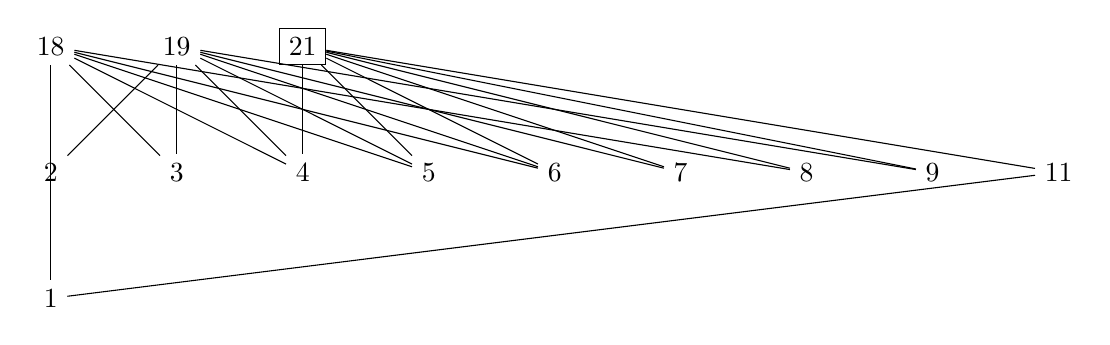
\begin{tikzpicture}
  \node[minimum size=0.3cm] (1) at (0.00,-3.20) {1};
  \node[minimum size=0.3cm] (2) at (0.00,-1.60) {2};
  \node[minimum size=0.3cm] (3) at (1.60,-1.60) {3};
  \node[minimum size=0.3cm] (4) at (3.20,-1.60) {4};
  \node[minimum size=0.3cm] (5) at (4.80,-1.60) {5};
  \node[minimum size=0.3cm] (6) at (6.40,-1.60) {6};
  \node[minimum size=0.3cm] (7) at (8.00,-1.60) {7};
  \node[minimum size=0.3cm] (8) at (9.60,-1.60) {8};
  \node[minimum size=0.3cm] (9) at (11.20,-1.60) {9};
  \node[minimum size=0.3cm] (11) at (12.80,-1.60) {11};
  \node[minimum size=0.3cm] (18) at (0.00,0.00) {18};
  \node[minimum size=0.3cm] (19) at (1.60,0.00) {19};
  \node[draw, rectangle, minimum size=0.3cm] (21) at (3.20,0.00) {21};
  % Draw the cover relations
  \draw (19) -- (6);
  \draw (19) -- (3);
  \draw (19) -- (9);
  \draw (18) -- (4);
  \draw (18) -- (1);
  \draw (21) -- (9);
  \draw (21) -- (6);
  \draw (19) -- (2);
  \draw (19) -- (5);
  \draw (11) -- (1);
  \draw (18) -- (3);
  \draw (18) -- (6);
  \draw (21) -- (5);
  \draw (21) -- (8);
  \draw (21) -- (11);
  \draw (19) -- (4);
  \draw (19) -- (7);
  \draw (18) -- (2);
  \draw (18) -- (5);
  \draw (21) -- (4);
  \draw (18) -- (8);
  \draw (21) -- (7);
\end{tikzpicture}
\end{minipage}%
\hfill\begin{minipage}{0.48\textwidth}
\subsubsection*{Void Poset}
\centering
\begin{tikzpicture}
  \node[minimum size=0.3cm] (18) at (0.00,0.00) {18};
  \node[draw, rectangle, minimum size=0.3cm] (19) at (1.60,0.00) {19};
  \node[minimum size=0.3cm] (2) at (0.00,-1.60) {2};
  \node[minimum size=0.3cm] (3) at (1.60,-1.60) {3};
  % Draw the cover relations
  \draw (19) -- (2);
  \draw (19) -- (3);
  \draw (18) -- (2);
  \draw (18) -- (3);
\end{tikzpicture}
\end{minipage}
\newpage\subsection{[8, 10, 12, 14, 17, 19]}
\noindent\begin{minipage}{0.6\textwidth}
\subsubsection*{Invariants}
\centering
\begin{tabular}{|c|c|c|c|c|c|c|}
\toprule
g & F & m & ewt & t & \(|M|\) & \(|\lambda|\) \\
\midrule
13 & 23 & 8 & 22 & 2 & 2 & 42 \\
\bottomrule
\end{tabular}
\end{minipage}%
\begin{minipage}{0.4\textwidth}
\subsubsection*{Partition}
\centering
\begin{tikzpicture}
  \draw (0.00, 0.00) rectangle (0.40, -0.40);
  \node[font=\tiny] at (0.20, -0.20) {23};
  \draw (0.40, 0.00) rectangle (0.80, -0.40);
  \node[font=\tiny] at (0.60, -0.20) {15};
  \draw (0.80, 0.00) rectangle (1.20, -0.40);
  \node[font=\tiny] at (1.00, -0.20) {13};
  \draw (1.20, 0.00) rectangle (1.60, -0.40);
  \node[font=\tiny] at (1.40, -0.20) {11};
  \draw (1.60, 0.00) rectangle (2.00, -0.40);
  \node[font=\tiny] at (1.80, -0.20) {9};
  \draw (2.00, 0.00) rectangle (2.40, -0.40);
  \node[font=\tiny] at (2.20, -0.20) {7};
  \draw (2.40, 0.00) rectangle (2.80, -0.40);
  \node[font=\tiny] at (2.60, -0.20) {6};
  \draw (2.80, 0.00) rectangle (3.20, -0.40);
  \node[font=\tiny] at (3.00, -0.20) {5};
  \draw (3.20, 0.00) rectangle (3.60, -0.40);
  \node[font=\tiny] at (3.40, -0.20) {4};
  \draw (3.60, 0.00) rectangle (4.00, -0.40);
  \node[font=\tiny] at (3.80, -0.20) {3};
  \draw (4.00, 0.00) rectangle (4.40, -0.40);
  \node[font=\tiny] at (4.20, -0.20) {1};
  \draw (0.00, -0.40) rectangle (0.40, -0.80);
  \node[font=\tiny] at (0.20, -0.60) {21};
  \draw (0.40, -0.40) rectangle (0.80, -0.80);
  \node[font=\tiny] at (0.60, -0.60) {13};
  \draw (0.80, -0.40) rectangle (1.20, -0.80);
  \node[font=\tiny] at (1.00, -0.60) {11};
  \draw (1.20, -0.40) rectangle (1.60, -0.80);
  \node[font=\tiny] at (1.40, -0.60) {9};
  \draw (1.60, -0.40) rectangle (2.00, -0.80);
  \node[font=\tiny] at (1.80, -0.60) {7};
  \draw (2.00, -0.40) rectangle (2.40, -0.80);
  \node[font=\tiny] at (2.20, -0.60) {5};
  \draw (2.40, -0.40) rectangle (2.80, -0.80);
  \node[font=\tiny] at (2.60, -0.60) {4};
  \draw (2.80, -0.40) rectangle (3.20, -0.80);
  \node[font=\tiny] at (3.00, -0.60) {3};
  \draw (3.20, -0.40) rectangle (3.60, -0.80);
  \node[font=\tiny] at (3.40, -0.60) {2};
  \draw (3.60, -0.40) rectangle (4.00, -0.80);
  \node[font=\tiny] at (3.80, -0.60) {1};
  \draw (0.00, -0.80) rectangle (0.40, -1.20);
  \node[font=\tiny] at (0.20, -1.00) {15};
  \draw (0.40, -0.80) rectangle (0.80, -1.20);
  \node[font=\tiny] at (0.60, -1.00) {7};
  \draw (0.80, -0.80) rectangle (1.20, -1.20);
  \node[font=\tiny] at (1.00, -1.00) {5};
  \draw (1.20, -0.80) rectangle (1.60, -1.20);
  \node[font=\tiny] at (1.40, -1.00) {3};
  \draw (1.60, -0.80) rectangle (2.00, -1.20);
  \node[font=\tiny] at (1.80, -1.00) {1};
  \draw (0.00, -1.20) rectangle (0.40, -1.60);
  \node[font=\tiny] at (0.20, -1.40) {13};
  \draw (0.40, -1.20) rectangle (0.80, -1.60);
  \node[font=\tiny] at (0.60, -1.40) {5};
  \draw (0.80, -1.20) rectangle (1.20, -1.60);
  \node[font=\tiny] at (1.00, -1.40) {3};
  \draw (1.20, -1.20) rectangle (1.60, -1.60);
  \node[font=\tiny] at (1.40, -1.40) {1};
  \draw (0.00, -1.60) rectangle (0.40, -2.00);
  \node[font=\tiny] at (0.20, -1.80) {11};
  \draw (0.40, -1.60) rectangle (0.80, -2.00);
  \node[font=\tiny] at (0.60, -1.80) {3};
  \draw (0.80, -1.60) rectangle (1.20, -2.00);
  \node[font=\tiny] at (1.00, -1.80) {1};
  \draw (0.00, -2.00) rectangle (0.40, -2.40);
  \node[font=\tiny] at (0.20, -2.20) {9};
  \draw (0.40, -2.00) rectangle (0.80, -2.40);
  \node[font=\tiny] at (0.60, -2.20) {1};
  \draw (0.00, -2.40) rectangle (0.40, -2.80);
  \node[font=\tiny] at (0.20, -2.60) {7};
  \draw (0.00, -2.80) rectangle (0.40, -3.20);
  \node[font=\tiny] at (0.20, -3.00) {6};
  \draw (0.00, -3.20) rectangle (0.40, -3.60);
  \node[font=\tiny] at (0.20, -3.40) {5};
  \draw (0.00, -3.60) rectangle (0.40, -4.00);
  \node[font=\tiny] at (0.20, -3.80) {4};
  \draw (0.00, -4.00) rectangle (0.40, -4.40);
  \node[font=\tiny] at (0.20, -4.20) {3};
  \draw (0.00, -4.40) rectangle (0.40, -4.80);
  \node[font=\tiny] at (0.20, -4.60) {2};
  \draw (0.00, -4.80) rectangle (0.40, -5.20);
  \node[font=\tiny] at (0.20, -5.00) {1};
\end{tikzpicture}
\end{minipage}
\vspace{1cm}
\noindent \newline\begin{minipage}{0.48\textwidth}
\subsubsection*{Gap Poset}
\centering
\begin{tikzpicture}
  \node[minimum size=0.3cm] (1) at (0.00,-3.20) {1};
  \node[minimum size=0.3cm] (3) at (1.60,-3.20) {3};
  \node[minimum size=0.3cm] (5) at (3.20,-3.20) {5};
  \node[minimum size=0.3cm] (7) at (4.80,-3.20) {7};
  \node[minimum size=0.3cm] (2) at (0.00,-1.60) {2};
  \node[minimum size=0.3cm] (4) at (1.60,-1.60) {4};
  \node[minimum size=0.3cm] (6) at (3.20,-1.60) {6};
  \node[minimum size=0.3cm] (9) at (4.80,-1.60) {9};
  \node[minimum size=0.3cm] (11) at (6.40,-1.60) {11};
  \node[minimum size=0.3cm] (13) at (8.00,-1.60) {13};
  \node[minimum size=0.3cm] (15) at (9.60,-1.60) {15};
  \node[minimum size=0.3cm] (21) at (0.00,0.00) {21};
  \node[draw, rectangle, minimum size=0.3cm] (23) at (1.60,0.00) {23};
  % Draw the cover relations
  \draw (23) -- (4);
  \draw (21) -- (13);
  \draw (23) -- (13);
  \draw (13) -- (5);
  \draw (15) -- (5);
  \draw (21) -- (9);
  \draw (23) -- (9);
  \draw (23) -- (6);
  \draw (23) -- (15);
  \draw (9) -- (1);
  \draw (11) -- (1);
  \draw (13) -- (1);
  \draw (15) -- (1);
  \draw (15) -- (7);
  \draw (21) -- (2);
  \draw (23) -- (11);
  \draw (21) -- (11);
  \draw (11) -- (3);
  \draw (13) -- (3);
  \draw (15) -- (3);
  \draw (21) -- (4);
  \draw (21) -- (7);
\end{tikzpicture}
\end{minipage}%
\hfill\begin{minipage}{0.48\textwidth}
\subsubsection*{Void Poset}
\centering
\begin{tikzpicture}
  \node[minimum size=0.3cm] (2) at (0.00,-1.60) {2};
  \node[draw, rectangle, minimum size=0.3cm] (21) at (0.00,0.00) {21};
  % Draw the cover relations
  \draw (21) -- (2);
\end{tikzpicture}
\end{minipage}
\newpage\subsection{[11, 13, 14, 15, 16, 17, 18, 19]}
\noindent\begin{minipage}{0.6\textwidth}
\subsubsection*{Invariants}
\centering
\begin{tabular}{|c|c|c|c|c|c|c|}
\toprule
g & F & m & ewt & t & \(|M|\) & \(|\lambda|\) \\
\midrule
14 & 23 & 11 & 25 & 3 & 4 & 40 \\
\bottomrule
\end{tabular}
\end{minipage}%
\begin{minipage}{0.4\textwidth}
\subsubsection*{Partition}
\centering
\begin{tikzpicture}
  \draw (0.00, 0.00) rectangle (0.40, -0.40);
  \node[font=\tiny] at (0.20, -0.20) {23};
  \draw (0.40, 0.00) rectangle (0.80, -0.40);
  \node[font=\tiny] at (0.60, -0.20) {12};
  \draw (0.80, 0.00) rectangle (1.20, -0.40);
  \node[font=\tiny] at (1.00, -0.20) {10};
  \draw (1.20, 0.00) rectangle (1.60, -0.40);
  \node[font=\tiny] at (1.40, -0.20) {9};
  \draw (1.60, 0.00) rectangle (2.00, -0.40);
  \node[font=\tiny] at (1.80, -0.20) {8};
  \draw (2.00, 0.00) rectangle (2.40, -0.40);
  \node[font=\tiny] at (2.20, -0.20) {7};
  \draw (2.40, 0.00) rectangle (2.80, -0.40);
  \node[font=\tiny] at (2.60, -0.20) {6};
  \draw (2.80, 0.00) rectangle (3.20, -0.40);
  \node[font=\tiny] at (3.00, -0.20) {5};
  \draw (3.20, 0.00) rectangle (3.60, -0.40);
  \node[font=\tiny] at (3.40, -0.20) {4};
  \draw (3.60, 0.00) rectangle (4.00, -0.40);
  \node[font=\tiny] at (3.80, -0.20) {1};
  \draw (0.00, -0.40) rectangle (0.40, -0.80);
  \node[font=\tiny] at (0.20, -0.60) {21};
  \draw (0.40, -0.40) rectangle (0.80, -0.80);
  \node[font=\tiny] at (0.60, -0.60) {10};
  \draw (0.80, -0.40) rectangle (1.20, -0.80);
  \node[font=\tiny] at (1.00, -0.60) {8};
  \draw (1.20, -0.40) rectangle (1.60, -0.80);
  \node[font=\tiny] at (1.40, -0.60) {7};
  \draw (1.60, -0.40) rectangle (2.00, -0.80);
  \node[font=\tiny] at (1.80, -0.60) {6};
  \draw (2.00, -0.40) rectangle (2.40, -0.80);
  \node[font=\tiny] at (2.20, -0.60) {5};
  \draw (2.40, -0.40) rectangle (2.80, -0.80);
  \node[font=\tiny] at (2.60, -0.60) {4};
  \draw (2.80, -0.40) rectangle (3.20, -0.80);
  \node[font=\tiny] at (3.00, -0.60) {3};
  \draw (3.20, -0.40) rectangle (3.60, -0.80);
  \node[font=\tiny] at (3.40, -0.60) {2};
  \draw (0.00, -0.80) rectangle (0.40, -1.20);
  \node[font=\tiny] at (0.20, -1.00) {20};
  \draw (0.40, -0.80) rectangle (0.80, -1.20);
  \node[font=\tiny] at (0.60, -1.00) {9};
  \draw (0.80, -0.80) rectangle (1.20, -1.20);
  \node[font=\tiny] at (1.00, -1.00) {7};
  \draw (1.20, -0.80) rectangle (1.60, -1.20);
  \node[font=\tiny] at (1.40, -1.00) {6};
  \draw (1.60, -0.80) rectangle (2.00, -1.20);
  \node[font=\tiny] at (1.80, -1.00) {5};
  \draw (2.00, -0.80) rectangle (2.40, -1.20);
  \node[font=\tiny] at (2.20, -1.00) {4};
  \draw (2.40, -0.80) rectangle (2.80, -1.20);
  \node[font=\tiny] at (2.60, -1.00) {3};
  \draw (2.80, -0.80) rectangle (3.20, -1.20);
  \node[font=\tiny] at (3.00, -1.00) {2};
  \draw (3.20, -0.80) rectangle (3.60, -1.20);
  \node[font=\tiny] at (3.40, -1.00) {1};
  \draw (0.00, -1.20) rectangle (0.40, -1.60);
  \node[font=\tiny] at (0.20, -1.40) {12};
  \draw (0.40, -1.20) rectangle (0.80, -1.60);
  \node[font=\tiny] at (0.60, -1.40) {1};
  \draw (0.00, -1.60) rectangle (0.40, -2.00);
  \node[font=\tiny] at (0.20, -1.80) {10};
  \draw (0.00, -2.00) rectangle (0.40, -2.40);
  \node[font=\tiny] at (0.20, -2.20) {9};
  \draw (0.00, -2.40) rectangle (0.40, -2.80);
  \node[font=\tiny] at (0.20, -2.60) {8};
  \draw (0.00, -2.80) rectangle (0.40, -3.20);
  \node[font=\tiny] at (0.20, -3.00) {7};
  \draw (0.00, -3.20) rectangle (0.40, -3.60);
  \node[font=\tiny] at (0.20, -3.40) {6};
  \draw (0.00, -3.60) rectangle (0.40, -4.00);
  \node[font=\tiny] at (0.20, -3.80) {5};
  \draw (0.00, -4.00) rectangle (0.40, -4.40);
  \node[font=\tiny] at (0.20, -4.20) {4};
  \draw (0.00, -4.40) rectangle (0.40, -4.80);
  \node[font=\tiny] at (0.20, -4.60) {3};
  \draw (0.00, -4.80) rectangle (0.40, -5.20);
  \node[font=\tiny] at (0.20, -5.00) {2};
  \draw (0.00, -5.20) rectangle (0.40, -5.60);
  \node[font=\tiny] at (0.20, -5.40) {1};
\end{tikzpicture}
\end{minipage}
\vspace{1cm}
\noindent \newline\begin{minipage}{0.48\textwidth}
\subsubsection*{Gap Poset}
\centering
\begin{tikzpicture}
  \node[minimum size=0.3cm] (1) at (0.00,-3.20) {1};
  \node[minimum size=0.3cm] (2) at (0.00,-1.60) {2};
  \node[minimum size=0.3cm] (3) at (1.60,-1.60) {3};
  \node[minimum size=0.3cm] (4) at (3.20,-1.60) {4};
  \node[minimum size=0.3cm] (5) at (4.80,-1.60) {5};
  \node[minimum size=0.3cm] (6) at (6.40,-1.60) {6};
  \node[minimum size=0.3cm] (7) at (8.00,-1.60) {7};
  \node[minimum size=0.3cm] (8) at (9.60,-1.60) {8};
  \node[minimum size=0.3cm] (9) at (11.20,-1.60) {9};
  \node[minimum size=0.3cm] (10) at (12.80,-1.60) {10};
  \node[minimum size=0.3cm] (12) at (14.40,-1.60) {12};
  \node[minimum size=0.3cm] (20) at (0.00,0.00) {20};
  \node[minimum size=0.3cm] (21) at (1.60,0.00) {21};
  \node[draw, rectangle, minimum size=0.3cm] (23) at (3.20,0.00) {23};
  % Draw the cover relations
  \draw (23) -- (4);
  \draw (20) -- (5);
  \draw (12) -- (1);
  \draw (23) -- (7);
  \draw (21) -- (10);
  \draw (23) -- (10);
  \draw (20) -- (4);
  \draw (21) -- (3);
  \draw (20) -- (1);
  \draw (20) -- (7);
  \draw (21) -- (6);
  \draw (23) -- (9);
  \draw (23) -- (6);
  \draw (23) -- (12);
  \draw (21) -- (2);
  \draw (20) -- (6);
  \draw (21) -- (5);
  \draw (20) -- (3);
  \draw (20) -- (9);
  \draw (21) -- (8);
  \draw (23) -- (5);
  \draw (23) -- (8);
  \draw (21) -- (4);
  \draw (20) -- (2);
  \draw (21) -- (7);
\end{tikzpicture}
\end{minipage}%
\hfill\begin{minipage}{0.48\textwidth}
\subsubsection*{Void Poset}
\centering
\begin{tikzpicture}
  \node[minimum size=0.3cm] (2) at (0.00,-1.60) {2};
  \node[minimum size=0.3cm] (3) at (1.60,-1.60) {3};
  \node[minimum size=0.3cm] (20) at (0.00,0.00) {20};
  \node[draw, rectangle, minimum size=0.3cm] (21) at (1.60,0.00) {21};
  % Draw the cover relations
  \draw (21) -- (2);
  \draw (21) -- (3);
  \draw (20) -- (2);
  \draw (20) -- (3);
\end{tikzpicture}
\end{minipage}
\newpage\subsection{[10, 12, 13, 14, 15, 16]}
\noindent\begin{minipage}{0.6\textwidth}
\subsubsection*{Invariants}
\centering
\begin{tabular}{|c|c|c|c|c|c|c|}
\toprule
g & F & m & ewt & t & \(|M|\) & \(|\lambda|\) \\
\midrule
14 & 21 & 10 & 25 & 4 & 6 & 40 \\
\bottomrule
\end{tabular}
\end{minipage}%
\begin{minipage}{0.4\textwidth}
\subsubsection*{Partition}
\centering
\begin{tikzpicture}
  \draw (0.00, 0.00) rectangle (0.40, -0.40);
  \node[font=\tiny] at (0.20, -0.20) {21};
  \draw (0.40, 0.00) rectangle (0.80, -0.40);
  \node[font=\tiny] at (0.60, -0.20) {11};
  \draw (0.80, 0.00) rectangle (1.20, -0.40);
  \node[font=\tiny] at (1.00, -0.20) {9};
  \draw (1.20, 0.00) rectangle (1.60, -0.40);
  \node[font=\tiny] at (1.40, -0.20) {8};
  \draw (1.60, 0.00) rectangle (2.00, -0.40);
  \node[font=\tiny] at (1.80, -0.20) {7};
  \draw (2.00, 0.00) rectangle (2.40, -0.40);
  \node[font=\tiny] at (2.20, -0.20) {6};
  \draw (2.40, 0.00) rectangle (2.80, -0.40);
  \node[font=\tiny] at (2.60, -0.20) {5};
  \draw (2.80, 0.00) rectangle (3.20, -0.40);
  \node[font=\tiny] at (3.00, -0.20) {1};
  \draw (0.00, -0.40) rectangle (0.40, -0.80);
  \node[font=\tiny] at (0.20, -0.60) {19};
  \draw (0.40, -0.40) rectangle (0.80, -0.80);
  \node[font=\tiny] at (0.60, -0.60) {9};
  \draw (0.80, -0.40) rectangle (1.20, -0.80);
  \node[font=\tiny] at (1.00, -0.60) {7};
  \draw (1.20, -0.40) rectangle (1.60, -0.80);
  \node[font=\tiny] at (1.40, -0.60) {6};
  \draw (1.60, -0.40) rectangle (2.00, -0.80);
  \node[font=\tiny] at (1.80, -0.60) {5};
  \draw (2.00, -0.40) rectangle (2.40, -0.80);
  \node[font=\tiny] at (2.20, -0.60) {4};
  \draw (2.40, -0.40) rectangle (2.80, -0.80);
  \node[font=\tiny] at (2.60, -0.60) {3};
  \draw (0.00, -0.80) rectangle (0.40, -1.20);
  \node[font=\tiny] at (0.20, -1.00) {18};
  \draw (0.40, -0.80) rectangle (0.80, -1.20);
  \node[font=\tiny] at (0.60, -1.00) {8};
  \draw (0.80, -0.80) rectangle (1.20, -1.20);
  \node[font=\tiny] at (1.00, -1.00) {6};
  \draw (1.20, -0.80) rectangle (1.60, -1.20);
  \node[font=\tiny] at (1.40, -1.00) {5};
  \draw (1.60, -0.80) rectangle (2.00, -1.20);
  \node[font=\tiny] at (1.80, -1.00) {4};
  \draw (2.00, -0.80) rectangle (2.40, -1.20);
  \node[font=\tiny] at (2.20, -1.00) {3};
  \draw (2.40, -0.80) rectangle (2.80, -1.20);
  \node[font=\tiny] at (2.60, -1.00) {2};
  \draw (0.00, -1.20) rectangle (0.40, -1.60);
  \node[font=\tiny] at (0.20, -1.40) {17};
  \draw (0.40, -1.20) rectangle (0.80, -1.60);
  \node[font=\tiny] at (0.60, -1.40) {7};
  \draw (0.80, -1.20) rectangle (1.20, -1.60);
  \node[font=\tiny] at (1.00, -1.40) {5};
  \draw (1.20, -1.20) rectangle (1.60, -1.60);
  \node[font=\tiny] at (1.40, -1.40) {4};
  \draw (1.60, -1.20) rectangle (2.00, -1.60);
  \node[font=\tiny] at (1.80, -1.40) {3};
  \draw (2.00, -1.20) rectangle (2.40, -1.60);
  \node[font=\tiny] at (2.20, -1.40) {2};
  \draw (2.40, -1.20) rectangle (2.80, -1.60);
  \node[font=\tiny] at (2.60, -1.40) {1};
  \draw (0.00, -1.60) rectangle (0.40, -2.00);
  \node[font=\tiny] at (0.20, -1.80) {11};
  \draw (0.40, -1.60) rectangle (0.80, -2.00);
  \node[font=\tiny] at (0.60, -1.80) {1};
  \draw (0.00, -2.00) rectangle (0.40, -2.40);
  \node[font=\tiny] at (0.20, -2.20) {9};
  \draw (0.00, -2.40) rectangle (0.40, -2.80);
  \node[font=\tiny] at (0.20, -2.60) {8};
  \draw (0.00, -2.80) rectangle (0.40, -3.20);
  \node[font=\tiny] at (0.20, -3.00) {7};
  \draw (0.00, -3.20) rectangle (0.40, -3.60);
  \node[font=\tiny] at (0.20, -3.40) {6};
  \draw (0.00, -3.60) rectangle (0.40, -4.00);
  \node[font=\tiny] at (0.20, -3.80) {5};
  \draw (0.00, -4.00) rectangle (0.40, -4.40);
  \node[font=\tiny] at (0.20, -4.20) {4};
  \draw (0.00, -4.40) rectangle (0.40, -4.80);
  \node[font=\tiny] at (0.20, -4.60) {3};
  \draw (0.00, -4.80) rectangle (0.40, -5.20);
  \node[font=\tiny] at (0.20, -5.00) {2};
  \draw (0.00, -5.20) rectangle (0.40, -5.60);
  \node[font=\tiny] at (0.20, -5.40) {1};
\end{tikzpicture}
\end{minipage}
\vspace{1cm}
\noindent \newline\begin{minipage}{0.48\textwidth}
\subsubsection*{Gap Poset}
\centering
\begin{tikzpicture}
  \node[minimum size=0.3cm] (1) at (0.00,-3.20) {1};
  \node[minimum size=0.3cm] (2) at (0.00,-1.60) {2};
  \node[minimum size=0.3cm] (3) at (1.60,-1.60) {3};
  \node[minimum size=0.3cm] (4) at (3.20,-1.60) {4};
  \node[minimum size=0.3cm] (5) at (4.80,-1.60) {5};
  \node[minimum size=0.3cm] (6) at (6.40,-1.60) {6};
  \node[minimum size=0.3cm] (7) at (8.00,-1.60) {7};
  \node[minimum size=0.3cm] (8) at (9.60,-1.60) {8};
  \node[minimum size=0.3cm] (9) at (11.20,-1.60) {9};
  \node[minimum size=0.3cm] (11) at (12.80,-1.60) {11};
  \node[minimum size=0.3cm] (17) at (0.00,0.00) {17};
  \node[minimum size=0.3cm] (18) at (1.60,0.00) {18};
  \node[minimum size=0.3cm] (19) at (3.20,0.00) {19};
  \node[draw, rectangle, minimum size=0.3cm] (21) at (4.80,0.00) {21};
  % Draw the cover relations
  \draw (17) -- (3);
  \draw (19) -- (6);
  \draw (19) -- (3);
  \draw (19) -- (9);
  \draw (18) -- (4);
  \draw (21) -- (9);
  \draw (21) -- (6);
  \draw (17) -- (2);
  \draw (17) -- (5);
  \draw (19) -- (5);
  \draw (11) -- (1);
  \draw (18) -- (3);
  \draw (18) -- (6);
  \draw (21) -- (5);
  \draw (21) -- (8);
  \draw (21) -- (11);
  \draw (17) -- (4);
  \draw (17) -- (1);
  \draw (17) -- (7);
  \draw (19) -- (4);
  \draw (19) -- (7);
  \draw (18) -- (2);
  \draw (18) -- (5);
  \draw (18) -- (8);
  \draw (21) -- (7);
\end{tikzpicture}
\end{minipage}%
\hfill\begin{minipage}{0.48\textwidth}
\subsubsection*{Void Poset}
\centering
\begin{tikzpicture}
  \node[minimum size=0.3cm] (2) at (0.00,-1.60) {2};
  \node[minimum size=0.3cm] (3) at (1.60,-1.60) {3};
  \node[minimum size=0.3cm] (4) at (3.20,-1.60) {4};
  \node[minimum size=0.3cm] (17) at (0.00,0.00) {17};
  \node[minimum size=0.3cm] (18) at (1.60,0.00) {18};
  \node[draw, rectangle, minimum size=0.3cm] (19) at (3.20,0.00) {19};
  % Draw the cover relations
  \draw (18) -- (4);
  \draw (19) -- (4);
  \draw (17) -- (3);
  \draw (18) -- (3);
  \draw (19) -- (3);
  \draw (17) -- (2);
  \draw (18) -- (2);
  \draw (17) -- (4);
\end{tikzpicture}
\end{minipage}
\newpage\subsection{[9, 10, 11, 12, 25]}
\noindent\begin{minipage}{0.6\textwidth}
\subsubsection*{Invariants}
\centering
\begin{tabular}{|c|c|c|c|c|c|c|}
\toprule
g & F & m & ewt & t & \(|M|\) & \(|\lambda|\) \\
\midrule
14 & 26 & 9 & 25 & 2 & 1 & 46 \\
\bottomrule
\end{tabular}
\end{minipage}%
\begin{minipage}{0.4\textwidth}
\subsubsection*{Partition}
\centering
\begin{tikzpicture}
  \draw (0.00, 0.00) rectangle (0.40, -0.40);
  \node[font=\tiny] at (0.20, -0.20) {26};
  \draw (0.40, 0.00) rectangle (0.80, -0.40);
  \node[font=\tiny] at (0.60, -0.20) {17};
  \draw (0.80, 0.00) rectangle (1.20, -0.40);
  \node[font=\tiny] at (1.00, -0.20) {16};
  \draw (1.20, 0.00) rectangle (1.60, -0.40);
  \node[font=\tiny] at (1.40, -0.20) {15};
  \draw (1.60, 0.00) rectangle (2.00, -0.40);
  \node[font=\tiny] at (1.80, -0.20) {14};
  \draw (2.00, 0.00) rectangle (2.40, -0.40);
  \node[font=\tiny] at (2.20, -0.20) {8};
  \draw (2.40, 0.00) rectangle (2.80, -0.40);
  \node[font=\tiny] at (2.60, -0.20) {7};
  \draw (2.80, 0.00) rectangle (3.20, -0.40);
  \node[font=\tiny] at (3.00, -0.20) {6};
  \draw (3.20, 0.00) rectangle (3.60, -0.40);
  \node[font=\tiny] at (3.40, -0.20) {5};
  \draw (3.60, 0.00) rectangle (4.00, -0.40);
  \node[font=\tiny] at (3.80, -0.20) {4};
  \draw (4.00, 0.00) rectangle (4.40, -0.40);
  \node[font=\tiny] at (4.20, -0.20) {3};
  \draw (4.40, 0.00) rectangle (4.80, -0.40);
  \node[font=\tiny] at (4.60, -0.20) {2};
  \draw (4.80, 0.00) rectangle (5.20, -0.40);
  \node[font=\tiny] at (5.00, -0.20) {1};
  \draw (0.00, -0.40) rectangle (0.40, -0.80);
  \node[font=\tiny] at (0.20, -0.60) {17};
  \draw (0.40, -0.40) rectangle (0.80, -0.80);
  \node[font=\tiny] at (0.60, -0.60) {8};
  \draw (0.80, -0.40) rectangle (1.20, -0.80);
  \node[font=\tiny] at (1.00, -0.60) {7};
  \draw (1.20, -0.40) rectangle (1.60, -0.80);
  \node[font=\tiny] at (1.40, -0.60) {6};
  \draw (1.60, -0.40) rectangle (2.00, -0.80);
  \node[font=\tiny] at (1.80, -0.60) {5};
  \draw (0.00, -0.80) rectangle (0.40, -1.20);
  \node[font=\tiny] at (0.20, -1.00) {16};
  \draw (0.40, -0.80) rectangle (0.80, -1.20);
  \node[font=\tiny] at (0.60, -1.00) {7};
  \draw (0.80, -0.80) rectangle (1.20, -1.20);
  \node[font=\tiny] at (1.00, -1.00) {6};
  \draw (1.20, -0.80) rectangle (1.60, -1.20);
  \node[font=\tiny] at (1.40, -1.00) {5};
  \draw (1.60, -0.80) rectangle (2.00, -1.20);
  \node[font=\tiny] at (1.80, -1.00) {4};
  \draw (0.00, -1.20) rectangle (0.40, -1.60);
  \node[font=\tiny] at (0.20, -1.40) {15};
  \draw (0.40, -1.20) rectangle (0.80, -1.60);
  \node[font=\tiny] at (0.60, -1.40) {6};
  \draw (0.80, -1.20) rectangle (1.20, -1.60);
  \node[font=\tiny] at (1.00, -1.40) {5};
  \draw (1.20, -1.20) rectangle (1.60, -1.60);
  \node[font=\tiny] at (1.40, -1.40) {4};
  \draw (1.60, -1.20) rectangle (2.00, -1.60);
  \node[font=\tiny] at (1.80, -1.40) {3};
  \draw (0.00, -1.60) rectangle (0.40, -2.00);
  \node[font=\tiny] at (0.20, -1.80) {14};
  \draw (0.40, -1.60) rectangle (0.80, -2.00);
  \node[font=\tiny] at (0.60, -1.80) {5};
  \draw (0.80, -1.60) rectangle (1.20, -2.00);
  \node[font=\tiny] at (1.00, -1.80) {4};
  \draw (1.20, -1.60) rectangle (1.60, -2.00);
  \node[font=\tiny] at (1.40, -1.80) {3};
  \draw (1.60, -1.60) rectangle (2.00, -2.00);
  \node[font=\tiny] at (1.80, -1.80) {2};
  \draw (0.00, -2.00) rectangle (0.40, -2.40);
  \node[font=\tiny] at (0.20, -2.20) {13};
  \draw (0.40, -2.00) rectangle (0.80, -2.40);
  \node[font=\tiny] at (0.60, -2.20) {4};
  \draw (0.80, -2.00) rectangle (1.20, -2.40);
  \node[font=\tiny] at (1.00, -2.20) {3};
  \draw (1.20, -2.00) rectangle (1.60, -2.40);
  \node[font=\tiny] at (1.40, -2.20) {2};
  \draw (1.60, -2.00) rectangle (2.00, -2.40);
  \node[font=\tiny] at (1.80, -2.20) {1};
  \draw (0.00, -2.40) rectangle (0.40, -2.80);
  \node[font=\tiny] at (0.20, -2.60) {8};
  \draw (0.00, -2.80) rectangle (0.40, -3.20);
  \node[font=\tiny] at (0.20, -3.00) {7};
  \draw (0.00, -3.20) rectangle (0.40, -3.60);
  \node[font=\tiny] at (0.20, -3.40) {6};
  \draw (0.00, -3.60) rectangle (0.40, -4.00);
  \node[font=\tiny] at (0.20, -3.80) {5};
  \draw (0.00, -4.00) rectangle (0.40, -4.40);
  \node[font=\tiny] at (0.20, -4.20) {4};
  \draw (0.00, -4.40) rectangle (0.40, -4.80);
  \node[font=\tiny] at (0.20, -4.60) {3};
  \draw (0.00, -4.80) rectangle (0.40, -5.20);
  \node[font=\tiny] at (0.20, -5.00) {2};
  \draw (0.00, -5.20) rectangle (0.40, -5.60);
  \node[font=\tiny] at (0.20, -5.40) {1};
\end{tikzpicture}
\end{minipage}
\vspace{1cm}
\noindent \newline\begin{minipage}{0.48\textwidth}
\subsubsection*{Gap Poset}
\centering
\begin{tikzpicture}
  \node[minimum size=0.3cm] (1) at (0.00,-1.60) {1};
  \node[minimum size=0.3cm] (14) at (1.60,-1.60) {14};
  \node[minimum size=0.3cm] (15) at (3.20,-1.60) {15};
  \node[minimum size=0.3cm] (16) at (4.80,-1.60) {16};
  \node[minimum size=0.3cm] (17) at (6.40,-1.60) {17};
  \node[minimum size=0.3cm] (2) at (0.00,-3.20) {2};
  \node[minimum size=0.3cm] (3) at (1.60,-3.20) {3};
  \node[minimum size=0.3cm] (4) at (3.20,-3.20) {4};
  \node[minimum size=0.3cm] (5) at (4.80,-3.20) {5};
  \node[minimum size=0.3cm] (6) at (6.40,-3.20) {6};
  \node[minimum size=0.3cm] (7) at (8.00,-3.20) {7};
  \node[minimum size=0.3cm] (8) at (9.60,-3.20) {8};
  \node[minimum size=0.3cm] (13) at (0.00,0.00) {13};
  \node[draw, rectangle, minimum size=0.3cm] (26) at (1.60,0.00) {26};
  % Draw the cover relations
  \draw (14) -- (4);
  \draw (17) -- (6);
  \draw (13) -- (2);
  \draw (16) -- (4);
  \draw (16) -- (7);
  \draw (15) -- (5);
  \draw (26) -- (14);
  \draw (26) -- (17);
  \draw (14) -- (3);
  \draw (17) -- (5);
  \draw (17) -- (8);
  \draw (13) -- (4);
  \draw (26) -- (1);
  \draw (13) -- (1);
  \draw (15) -- (4);
  \draw (16) -- (6);
  \draw (26) -- (16);
  \draw (14) -- (2);
  \draw (14) -- (5);
  \draw (17) -- (7);
  \draw (13) -- (3);
  \draw (15) -- (6);
  \draw (16) -- (5);
  \draw (15) -- (3);
  \draw (26) -- (15);
\end{tikzpicture}
\end{minipage}%
\hfill\begin{minipage}{0.48\textwidth}
\subsubsection*{Void Poset}
\centering
\begin{tikzpicture}
  \node[draw, rectangle, minimum size=0.3cm] (13) at (0.00,0.00) {13};
\end{tikzpicture}
\end{minipage}
\newpage\subsection{[8, 10, 12, 14, 17]}
\noindent\begin{minipage}{0.6\textwidth}
\subsubsection*{Invariants}
\centering
\begin{tabular}{|c|c|c|c|c|c|c|}
\toprule
g & F & m & ewt & t & \(|M|\) & \(|\lambda|\) \\
\midrule
14 & 23 & 8 & 25 & 3 & 4 & 48 \\
\bottomrule
\end{tabular}
\end{minipage}%
\begin{minipage}{0.4\textwidth}
\subsubsection*{Partition}
\centering
\begin{tikzpicture}
  \draw (0.00, 0.00) rectangle (0.40, -0.40);
  \node[font=\tiny] at (0.20, -0.20) {23};
  \draw (0.40, 0.00) rectangle (0.80, -0.40);
  \node[font=\tiny] at (0.60, -0.20) {15};
  \draw (0.80, 0.00) rectangle (1.20, -0.40);
  \node[font=\tiny] at (1.00, -0.20) {13};
  \draw (1.20, 0.00) rectangle (1.60, -0.40);
  \node[font=\tiny] at (1.40, -0.20) {11};
  \draw (1.60, 0.00) rectangle (2.00, -0.40);
  \node[font=\tiny] at (1.80, -0.20) {9};
  \draw (2.00, 0.00) rectangle (2.40, -0.40);
  \node[font=\tiny] at (2.20, -0.20) {7};
  \draw (2.40, 0.00) rectangle (2.80, -0.40);
  \node[font=\tiny] at (2.60, -0.20) {6};
  \draw (2.80, 0.00) rectangle (3.20, -0.40);
  \node[font=\tiny] at (3.00, -0.20) {5};
  \draw (3.20, 0.00) rectangle (3.60, -0.40);
  \node[font=\tiny] at (3.40, -0.20) {3};
  \draw (3.60, 0.00) rectangle (4.00, -0.40);
  \node[font=\tiny] at (3.80, -0.20) {1};
  \draw (0.00, -0.40) rectangle (0.40, -0.80);
  \node[font=\tiny] at (0.20, -0.60) {21};
  \draw (0.40, -0.40) rectangle (0.80, -0.80);
  \node[font=\tiny] at (0.60, -0.60) {13};
  \draw (0.80, -0.40) rectangle (1.20, -0.80);
  \node[font=\tiny] at (1.00, -0.60) {11};
  \draw (1.20, -0.40) rectangle (1.60, -0.80);
  \node[font=\tiny] at (1.40, -0.60) {9};
  \draw (1.60, -0.40) rectangle (2.00, -0.80);
  \node[font=\tiny] at (1.80, -0.60) {7};
  \draw (2.00, -0.40) rectangle (2.40, -0.80);
  \node[font=\tiny] at (2.20, -0.60) {5};
  \draw (2.40, -0.40) rectangle (2.80, -0.80);
  \node[font=\tiny] at (2.60, -0.60) {4};
  \draw (2.80, -0.40) rectangle (3.20, -0.80);
  \node[font=\tiny] at (3.00, -0.60) {3};
  \draw (3.20, -0.40) rectangle (3.60, -0.80);
  \node[font=\tiny] at (3.40, -0.60) {1};
  \draw (0.00, -0.80) rectangle (0.40, -1.20);
  \node[font=\tiny] at (0.20, -1.00) {19};
  \draw (0.40, -0.80) rectangle (0.80, -1.20);
  \node[font=\tiny] at (0.60, -1.00) {11};
  \draw (0.80, -0.80) rectangle (1.20, -1.20);
  \node[font=\tiny] at (1.00, -1.00) {9};
  \draw (1.20, -0.80) rectangle (1.60, -1.20);
  \node[font=\tiny] at (1.40, -1.00) {7};
  \draw (1.60, -0.80) rectangle (2.00, -1.20);
  \node[font=\tiny] at (1.80, -1.00) {5};
  \draw (2.00, -0.80) rectangle (2.40, -1.20);
  \node[font=\tiny] at (2.20, -1.00) {3};
  \draw (2.40, -0.80) rectangle (2.80, -1.20);
  \node[font=\tiny] at (2.60, -1.00) {2};
  \draw (2.80, -0.80) rectangle (3.20, -1.20);
  \node[font=\tiny] at (3.00, -1.00) {1};
  \draw (0.00, -1.20) rectangle (0.40, -1.60);
  \node[font=\tiny] at (0.20, -1.40) {15};
  \draw (0.40, -1.20) rectangle (0.80, -1.60);
  \node[font=\tiny] at (0.60, -1.40) {7};
  \draw (0.80, -1.20) rectangle (1.20, -1.60);
  \node[font=\tiny] at (1.00, -1.40) {5};
  \draw (1.20, -1.20) rectangle (1.60, -1.60);
  \node[font=\tiny] at (1.40, -1.40) {3};
  \draw (1.60, -1.20) rectangle (2.00, -1.60);
  \node[font=\tiny] at (1.80, -1.40) {1};
  \draw (0.00, -1.60) rectangle (0.40, -2.00);
  \node[font=\tiny] at (0.20, -1.80) {13};
  \draw (0.40, -1.60) rectangle (0.80, -2.00);
  \node[font=\tiny] at (0.60, -1.80) {5};
  \draw (0.80, -1.60) rectangle (1.20, -2.00);
  \node[font=\tiny] at (1.00, -1.80) {3};
  \draw (1.20, -1.60) rectangle (1.60, -2.00);
  \node[font=\tiny] at (1.40, -1.80) {1};
  \draw (0.00, -2.00) rectangle (0.40, -2.40);
  \node[font=\tiny] at (0.20, -2.20) {11};
  \draw (0.40, -2.00) rectangle (0.80, -2.40);
  \node[font=\tiny] at (0.60, -2.20) {3};
  \draw (0.80, -2.00) rectangle (1.20, -2.40);
  \node[font=\tiny] at (1.00, -2.20) {1};
  \draw (0.00, -2.40) rectangle (0.40, -2.80);
  \node[font=\tiny] at (0.20, -2.60) {9};
  \draw (0.40, -2.40) rectangle (0.80, -2.80);
  \node[font=\tiny] at (0.60, -2.60) {1};
  \draw (0.00, -2.80) rectangle (0.40, -3.20);
  \node[font=\tiny] at (0.20, -3.00) {7};
  \draw (0.00, -3.20) rectangle (0.40, -3.60);
  \node[font=\tiny] at (0.20, -3.40) {6};
  \draw (0.00, -3.60) rectangle (0.40, -4.00);
  \node[font=\tiny] at (0.20, -3.80) {5};
  \draw (0.00, -4.00) rectangle (0.40, -4.40);
  \node[font=\tiny] at (0.20, -4.20) {4};
  \draw (0.00, -4.40) rectangle (0.40, -4.80);
  \node[font=\tiny] at (0.20, -4.60) {3};
  \draw (0.00, -4.80) rectangle (0.40, -5.20);
  \node[font=\tiny] at (0.20, -5.00) {2};
  \draw (0.00, -5.20) rectangle (0.40, -5.60);
  \node[font=\tiny] at (0.20, -5.40) {1};
\end{tikzpicture}
\end{minipage}
\vspace{1cm}
\noindent \newline\begin{minipage}{0.48\textwidth}
\subsubsection*{Gap Poset}
\centering
\begin{tikzpicture}
  \node[minimum size=0.3cm] (1) at (0.00,-3.20) {1};
  \node[minimum size=0.3cm] (3) at (1.60,-3.20) {3};
  \node[minimum size=0.3cm] (5) at (3.20,-3.20) {5};
  \node[minimum size=0.3cm] (7) at (4.80,-3.20) {7};
  \node[minimum size=0.3cm] (2) at (0.00,-1.60) {2};
  \node[minimum size=0.3cm] (4) at (1.60,-1.60) {4};
  \node[minimum size=0.3cm] (6) at (3.20,-1.60) {6};
  \node[minimum size=0.3cm] (9) at (4.80,-1.60) {9};
  \node[minimum size=0.3cm] (11) at (6.40,-1.60) {11};
  \node[minimum size=0.3cm] (13) at (8.00,-1.60) {13};
  \node[minimum size=0.3cm] (15) at (9.60,-1.60) {15};
  \node[minimum size=0.3cm] (19) at (0.00,0.00) {19};
  \node[minimum size=0.3cm] (21) at (1.60,0.00) {21};
  \node[draw, rectangle, minimum size=0.3cm] (23) at (3.20,0.00) {23};
  % Draw the cover relations
  \draw (21) -- (13);
  \draw (23) -- (13);
  \draw (19) -- (9);
  \draw (13) -- (5);
  \draw (15) -- (5);
  \draw (21) -- (9);
  \draw (23) -- (9);
  \draw (23) -- (6);
  \draw (23) -- (15);
  \draw (19) -- (2);
  \draw (9) -- (1);
  \draw (19) -- (5);
  \draw (19) -- (11);
  \draw (11) -- (1);
  \draw (13) -- (1);
  \draw (15) -- (1);
  \draw (15) -- (7);
  \draw (23) -- (11);
  \draw (21) -- (11);
  \draw (19) -- (7);
  \draw (11) -- (3);
  \draw (13) -- (3);
  \draw (15) -- (3);
  \draw (21) -- (4);
  \draw (21) -- (7);
\end{tikzpicture}
\end{minipage}%
\hfill\begin{minipage}{0.48\textwidth}
\subsubsection*{Void Poset}
\centering
\begin{tikzpicture}
  \node[minimum size=0.3cm] (2) at (0.00,-1.60) {2};
  \node[minimum size=0.3cm] (4) at (1.60,-1.60) {4};
  \node[minimum size=0.3cm] (19) at (0.00,0.00) {19};
  \node[draw, rectangle, minimum size=0.3cm] (21) at (1.60,0.00) {21};
  % Draw the cover relations
  \draw (19) -- (2);
  \draw (21) -- (4);
\end{tikzpicture}
\end{minipage}
\end{document}
